\documentclass{book}

\usepackage{graphicx}
%\usepackage{multirow}
%\usepackage{bm} %% bold face math symbols
\usepackage{listings}
\usepackage{../macros/mytikz}
\usetikzlibrary{shapes}
%\usepackage{stmaryrd}%\newcommand{\contra}{\lightning}
%\usepackage{rotating} \newcommand{\sw}[1]{\begin{sideways}#1\end{sideways}}

\usepackage{../macros/algorithm}
%\usepackage{ded}
\usepackage{../mylecturenotes}

\title{Lectures Notes on Secure and Dependable Systems}
\author{Florian Rabe}
\date{2017}


\begin{document}
\maketitle

\tableofcontents
\newpage

\part{Introduction}

 \chapter{Meta-Remarks}
  \begin{center}
\textbf{Important stuff that you should read carefully!}
\end{center}

\paragraph{State of these notes}
I constantly work on my lecture notes.
Therefore, keep in mind that:
\begin{compactitem}
\item I am developing these notes in parallel with the lecture---they can grow or change throughout the semester.
\item These notes are neither a subset nor a superset of the material discussed in the lecture.
\item Unless mentioned otherwise, all material in these notes is exam-relevant (in addition to all material discussed in the lectures).
\end{compactitem}
\medskip

\paragraph{Collaboration on these notes}
I am writing these notes using LaTeX and storing them in a git repository on GitHub at \cite{}.
Familiarity with LaTeX as well as Git and GitHub is not part of this lecture. But it is essential skill for you.
Ask in the lecture if you have difficulty figuring it out on your own.
\medskip

As an experiment in teaching, I am inviting all of you to collaborate on these lecture notes with me.
\medskip

By forking and by submitting pull requests for this repository, you can suggest changes to these notes.
For example, you are encouraged to:
\begin{compactitem}
\item Fix typos and other errors.
\item Add examples and diagrams that I develop on the board during lectures.
\item Add solutions for the homeworks if I did not provide any (of course, I will only integrate solutions after the deadline).
\item Add additional examples, exercises, or explanations that you came up or found in other sources.
 If you use material from other sources (e.g., by copying an diagram from some website), make sure that you have the license to use it and that you acknowledge sources appropriately!
\end{compactitem}
The TAs and I will review and approve or reject the changes.
If you make substantial contributions, I will list you as a contributor (i.e., something you can put in your CV).
\medskip

Any improvement you make will not only help your fellow students, it will also increase your own understanding of the material.
Therefore, I can give you up to $10\%$ bonus credit for such contributions.
(Make sure your git commits carry a user name that I can connect to you.)
Because this is an experiment, I will have to figure out the details along the way.

\paragraph{Other Advice}
I maintain a list of useful advice for students at \url{https://svn.kwarc.info/repos/frabe/Teaching/general/advice_for_students.pdf}.
It is mostly targeted at older students who work in individual projects with me (e.g., students who work on their BSc thesis).
But much of it is useful for you already now or will become useful soon.
So have a look.

  \chapter{Concepts}
   This section mostly follows \cite{dependability}, including some tables, which is available online.

Computer systems can be evaluated according to
\begin{compactitem}
 \item functionality
 \item usability
 \item performance
 \item cost
 \item dependability
\end{compactitem}

\textbf{Dependability} means to deliver service to a user that can justifiably be trusted.
The user is another system (physical or human) that interacts with the former at the service interface.
The \textbf{function} of a system is what the system is intended to do as described by its functional specification.
Correct service is delivered when the service implements the specification.

A systematic exposition of the concepts of dependability consists of three parts: the attributes of dependability, their threats, and means to achieve dependability.
An overview is given in Fig.~\ref{fig:concepts_dep}.

\begin{figure}
\centering
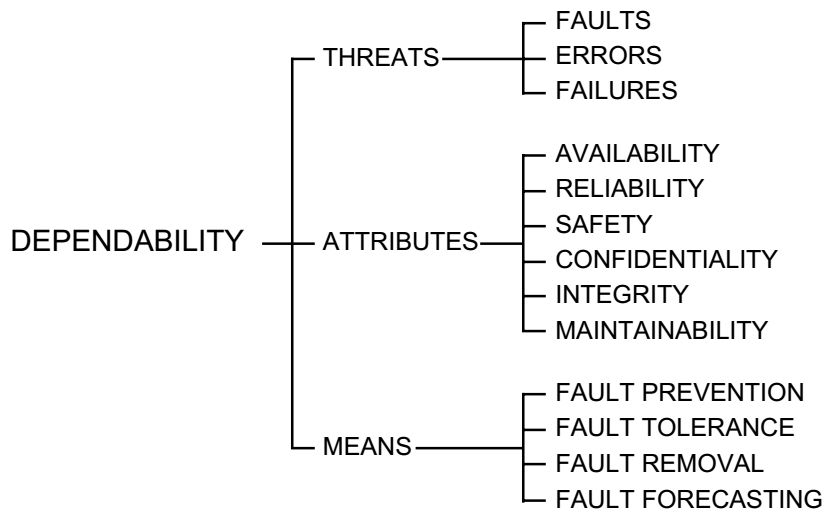
\includegraphics[width=0.7\linewidth]{concepts_dep}
%Latex does not support the incusion of .jpg files, only of .eps, .ps and .pdf (other stuff potentially depends on the latex distribution, this probably works only on miktex on windows)
\caption{Concepts Related to Dependability}
\label{fig:concepts_dep}
\end{figure}

\section{Attributes}

\subsection{Definitions}

\textbf{Availability} means the readiness for correct service.
This includes two subaspects: the functionality has to \textbf{exist} and be realized \textbf{correctly}, i.e., according to its specification.

\textbf{Reliability} means the continuity of correct service.
This is similar to availability but emphasizes that the service not only exists but exist without downtime or intermittent failures.

\textbf{Safety} means the absence of catastrophic consequences on the user(s) and the environment.
Often safety involves interpreting signals received from and sending signals to external devices that operate in the real world, e.g., the cameras and the engine of the car.
This introduces additional uncertainty (not to mention the other cars and pedestrians) that can be difficult to anticipate in the specification.

\textbf{Security} means the availability for authorized users only.
This includes protection against any malicious influenced from the outside, i.e., any kind of attack or hacking.
This includes all defenses against hacking.\footnote{\cite{dependability} calls a related property \emph{integrity}, and then defines security as the combination of integrity and confidentiality.}

\textbf{Confidentiality} means the absence of unauthorized disclosure of information.
This includes the security of all private data including any intermediate results of computation such as passwords or keys.

\textbf{Maintainability} means the ability to undergo repairs and modifications.
This includes all necessary changes needed during long-term deployment.

\subsection{Incomplete Specifications}

Often the attributes are not or only implicitly part of the specification of a system.

Availability is usually implicitly required, but details may be omitted.
For example, the acceptable variation of response times may be unspecified.

Reliability is also usually implicit required, but details may be omitted.
For example, the acceptable downtime may be unspecified.

Safety is usually specified well if a potential safety danger is realized.
But it can be easy to foresee all necessary safety requirements.

Security is often forgotten completely or partially.
It is usually difficult to translate the abstract requirement of security into concrete, testable properties.
After all, the first mistake of security is to assume to know what the attacker might do.

Confidentiality is often considered even less then security.

Maintainability is often ignored completely.
That is a typical pitfall for large projects, where realizing any requirement at deploy time may be completely different from realizing it after a year or later.
This is because intermediate changes have messed up the system so much that, e.g., security flaws are not noticed anymore.

\subsection{Imperfect Implementations}

All attributes are very difficult to realize perfectly in implementations.

Availability and reliability often fail.
In addition to plain design or implementation errors, there may be failures in hardware, networks, operating system, external components that were not foreseen by the developer.

Together with correctness, safety is the only property that is at least in principle accessible to a formal definition.
But the resulting problem is undecidable.
So in practice, we have to use extensive testing.  

Security is very complex to prove because any proof must make assumptions about what kind of attacks there are.
Attacking a system often requires intentionally violating the specification and supply unanticipated input.

Perfect confidentiality is impossible to realize because all computation leaks some information other than the output: This reaches from runtime and resource use to obscure effects like the development of heat due to CPU activity.

Maintainability is hard to realize because especially inexperienced developers or unskilled managers cannot assess whether a particular design is maintainable.

\section{Threats}

\subsection{Failures}

A system \textbf{failure} is an event that occurs when the delivered service deviates from correct service.
See Fig.~\ref{fig:concepts_fail} for an overview of related concepts.

A \textbf{fault} is the adjudged or hypothesized cause of an error.
A fault is \textbf{active} when it produces an error; otherwise it is \textbf{dormant}.
See Fig.~\ref{fig:concepts_fault} for an overview of related concepts.

An \textbf{error} is that part of the system state that may cause a subsequent failure: a failure occurs when an error reaches the service interface and alters the service.

\begin{figure}
\centering
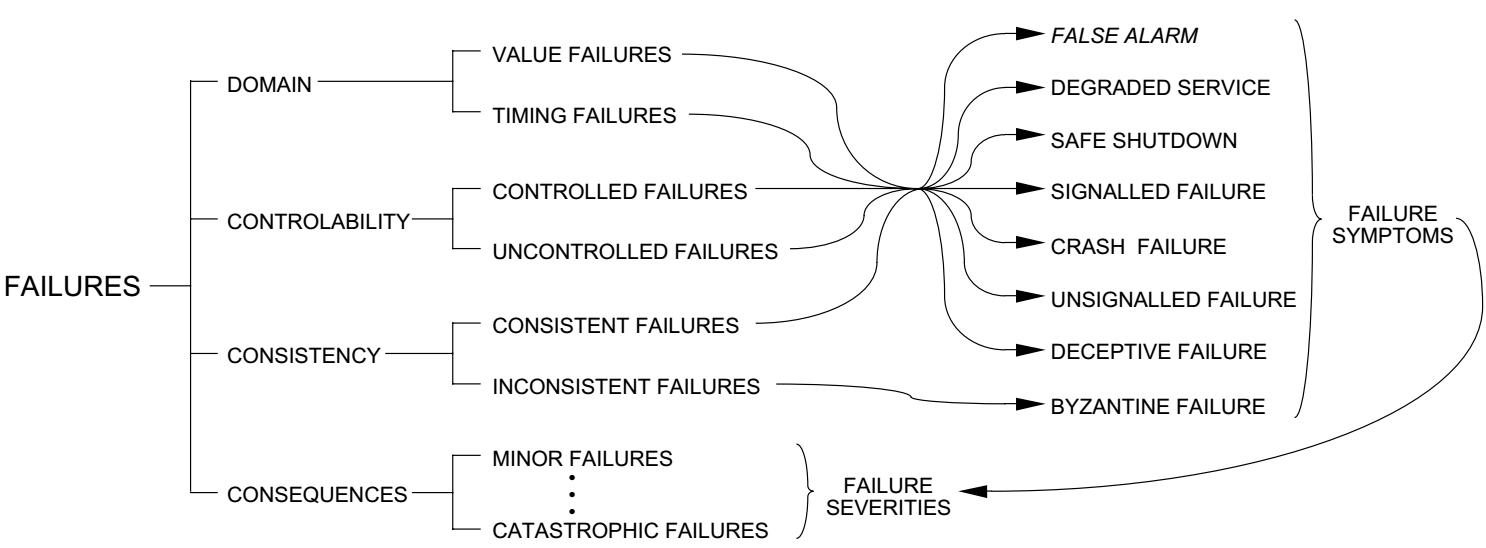
\includegraphics[width=0.7\linewidth]{concepts_fail}
\caption{Failure Modes}
\label{fig:concepts_fail}
\end{figure}

\begin{figure}
\centering
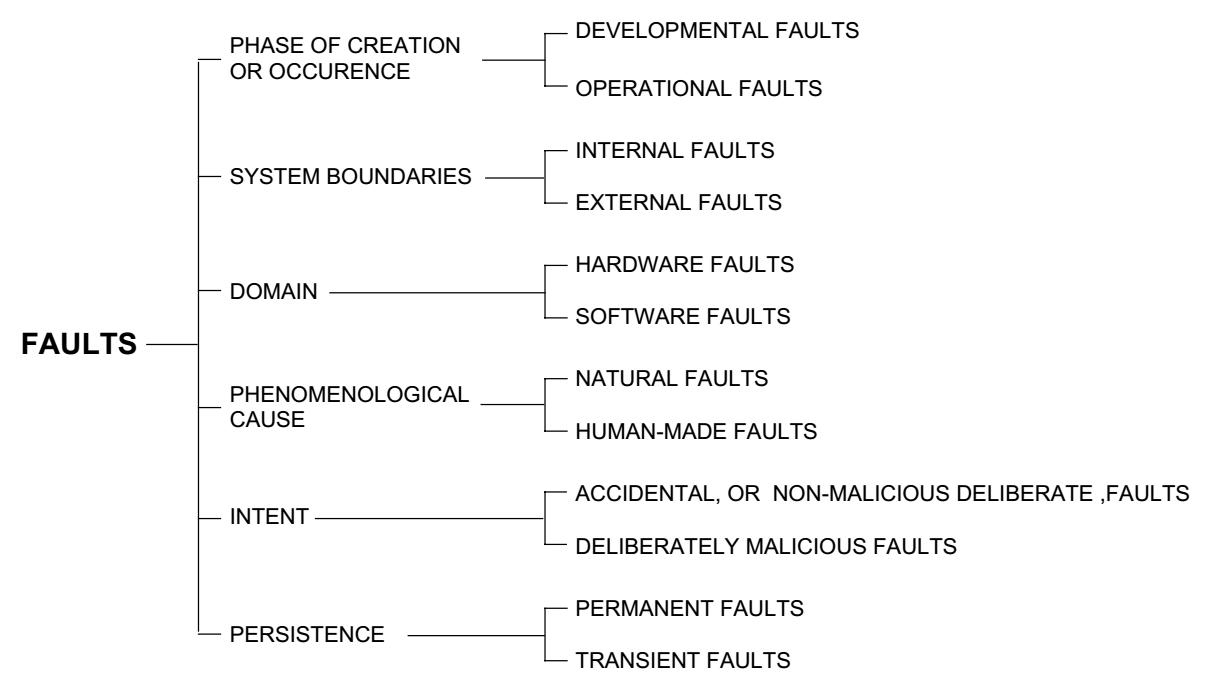
\includegraphics[width=0.7\linewidth]{concepts_fault}
\caption{Fault Classes}
\label{fig:concepts_fault}
\end{figure}

\section{Means}

\subsection{Fault Prevention}

Fault prevention requires quality control techniques employed during the design and manufacturing of the system.
That includes, e.g., structured programming, information hiding, or modularization.

Shielding, radiation hardening, etc., are needed to prevent physical faults.
Training and maintenance procedures aim at preventing interaction faults.
Firewalls and similar defenses intend to prevent malicious faults.

\subsection{Fault Tolerance}

Fault tolerance is intended to preserve the delivery of correct service in the presence of active faults.
This may refer to accidental or malicious faults.

\paragraph{Error detection}
An error that is present but not detected is a \textbf{latent} error. 
Concurrent error detection takes place during service delivery.
Preemptive error detection takes place while service delivery is suspended; it checks the
system for latent errors and dormant faults.

\paragraph{Recovery}
Recovery consists of error handling and fault handling.

Error handling eliminates errors from the system state by
\begin{compactitem}
  \item rollback: the state is transformed to a previously saved state
  \item compensation: the erroneous state is redundant enough to eliminate the error,
  \item rollforward: the state is transformed to a new state without the detected error.
\end{compactitem}

Fault handling prevents located faults from being activated again by
\begin{compactitem}
  \item fault diagnosis: identify location and type of the cause of an error
  \item fault isolation: exclude the fault from future service delivery, i.e., make the fault dormant
  \item system reconfiguration: switch to non-failed components
  \item system reinitialization: update to a new configuration of the system
\end{compactitem}

The choice of error detection, error handling, and fault handling techniques, and of their implementation, is directly related to the underlying fault assumption.

Fault tolerance is recursive: Its implementation must be protected against faults as well.


\subsection{Fault Removal}

\paragraph{Development Phase}
Fault removal during the development phase of a system consists of three steps:
\begin{compactitem}
 \item Verification checks whether the system satisfies required properties.
 \item If verification fails, diagnosis identifies the faults that prevented verification.
 \item After diagnosis, correction is carried, and verification repeated.
\end{compactitem}

Multiple different properties can be verified:
\begin{compactitem}
 \item Verifying the specification is usually referred to as validation.
Static verification does not exercise the systems and uses static analysis (e.g., inspections or walk-through), model-checking, or theorem proving.
Dynamic verification exercises the systems and uses testing.
\item Verifying the fault tolerance mechanism.
This can employ formal static verification or fault injection, i.e., testing where intentional faults or errors are part of the test.
\item Verifying that the system cannot do more than specified is especially relevant for safety and security.
\end{compactitem}

\emph{Design for verifiability} means to design a system in such a way that verification becomes easy.

\paragraph{Operation Phase}
Fault removal during the life time of a system employs two methods:
\begin{compactitem}
\item Corrective maintenance removes faults that have produced errors that were detected and reported.
\item Preventive maintenance uncovers faults before they cause errors.
This may also include design faults that have caused errors in similar systems.
\end{compactitem}

Fault removal during operation often first isolates the fault (e.g., by a workaround or patch) before the actual removal is carried out.

\subsection{Fault Forecasting}

Fault forecasting evaluates a system with respect to fault occurrence or activation.
It has two aspects:
\begin{compactitem}
  \item Qualitative evaluation identifies, classifies, and ranks the failure modes, or the event combinations that would lead to system failures.
  \item Quantitative evaluation determines the probabilities to which some of the attributes of dependability are satisfied, which are then viewed as measures of dependability.
  This may use, e.g., Markov chains or Petri nets.
\end{compactitem}

%Dependability can remain stable, grow, or decrease during a system's life-cycle.
%These can be measure by failure intensity, i.e., the number of failures per unit of time.
%It typically first decreases, then stabilizes, then increases, and the cycle resumes.
%
%The alternation of correct-incorrect service delivery is quantified to define reliability, availability, and maintainability as measures of dependability:
%\begin{compactitem}
% \item reliability: a measure of the continuous delivery of correct service---or, equivalently, of the time to failure,
% \item availability: a measure of the delivery of correct service with respect to the alternation of correct and incorrect service,
%• maintainability: a measure of the time to service restoration since the last failure occurrence, or
%equivalently, measure of the continuous delivery of incorrect service,
%• safety is an extension of reliability: when the state of correct service and the states of incorrect
%service due to non-catastrophic failure are grouped into a safe state (in the sense of being free from
%catastrophic damage, not from danger), safety is a measure of continuous safeness, or equivalently,
%of the time to catastrophic failure; safety is thus reliability with respect to catastrophic failures.
%Generally, a system delivers several services, and there often are two or more modes of service quality,
%e.g. ranging from full capacity to emergency service. These modes distinguish less and less complete
%service deliveries. Performance-related measures of dependability are usually subsumed into the notion
%of performability.

%The main approaches to derive probabilistic measures of dependability measures are modeling and testing.
%These approaches are complementary since modeling needs data on the basic processes modeled (failure process, maintenance process, system activation process, etc.), that may be obtained either by testing, or by the processing of failure data.
%When evaluating fault-tolerant systems, the effectiveness of error and fault handling mechanisms, i.e., their coverage, has a drastic influence on dependability measures.
%The evaluation of coverage can be performed either through modeling or through testing, i.e. fault injection.


 \chapter{Challenges}
   This chapter lists examples of disasters and failures that serve as examples of what secure and dependable systems should avoid.

The lists are not complete and may be biased by whether
\begin{compactitem}
 \item I became aware of it and found it interesting enough
 \item the cause could be determined and was made public
\end{compactitem}
Feel free to edit these notes by adding important examples that I forgot when I compiled the lists.

All damage estimates are relative to the time of the event and not adjusted to inflation.

Note that for security problems, the size of the damage is naturally unknown because attacks will typically remain secret.
Only the cost of updating the systems can be estimated, which may or may not be indicative of the severity of the security problem.

\section{General Aspects}

\highlightframe{
State-of-the-art software and hardware systems simply are not safe, secure, and dependable.

Moreover, we do not understand very well yet how to make them so.
}

This is different from many other areas such as mechanical or chemical engineering.
While these occasionally cause disasters, these can usually be traced back to human error, foul play, or negligent or intentional violation of regulations.
Such disasters usually result in criminal proceedings, civil litigation, or revision or extension of regulations.
% what engineers know and how they know it

The situation is very different for computer systems.
There is no general methodology for designing and operating computer systems well that can be easily described, taught, or codified.

The situation will hopefully improve over the course of the 21st century.
The problem has been recognized decades ago, and many companies and researchers are working on it.
They approach from very different directions with different goals and different methodologies.

\highlightframe{
This has resulted in a wide and diverse variety of not coherently connected methods with varying degrees of depth, maturity, cost, benefit, and practical adoption.
}

A typical effect is a trade-off along a spectrum of methods:
\begin{compactitem}
 \item cheap but weak methods on one end
 \item strong but expensive methods on the other end.
\end{compactitem}
Therefore, it is often necessary to choose a degree of safety assurance rather than actually guarantee safety.
This spectrum is so extreme that
\begin{compactitem}
 \item the majority of practical software development does not systematically ensure any kind of safety,
 \item the majority of theoretical solutions are neither ready nor affordable for practical use.
\end{compactitem}

Incidentally, this means that this course's subject matter is much less well-defined than that of other courses.%
\footnote{For example, the other two courses in this module almost design themselves because the subject matter is very well understood and standardized.}
That makes it particular difficult to design a syllabus for.
It will give an overview of the most important state-of-the-art methods.

\section{Major Disasters Caused by Programming Errors}

\paragraph{Space Exploration}
There have been a number of failures in space exploration due to minor programming errors.
These include
\begin{compactitem}
 \item 1962, Mariner 1 rocket lost: misread specification (overlooked bar over a variable) was implemented (damage around \$$20$ million)
 \item 1982, Viking I lost: software update written to wrong memory area overriding vital parameters for antenna
 \item 1988, Phobos 1 lost: one character missing in software update led to accidentally executing a testing routing at the wrong time
 \item 1996, Mars Global Surveyor lost: data written to wrong memory addresses
 \item 1999, Mars Polar Lander lost: presumably software not accounting for false positive when detecting shutdown even though the possibility was known
 \item 2004, Mars Rover Spirit lost for 16 days: delay in deleting obsolete files led to lack of available flash memory, which triggered a reboot, which led to a reboot cycle
\end{compactitem}
% the story of a Fortran bug where . was accidentally written instead of a , appears to be exaaggerated; it did not lead to a crash

\paragraph{Therac-25}
Between 1985 and 1987, the Therac-25 machine for medical radiation therapy caused death and/or serious injury in at least $6$ cases.
Patients received a radiation overdose because the high intensity energy beam was administered while using the protection meant for the low intensity beam.

The cause was that the hardware protection was discontinued, relying exclusively on software to prevent a mismatch of beam and protection configuration.
But the software had always been buggy due to a systemic failures in the software engineering process including complex systems (code written in assembly, machine had its own OS), lack of software review, insufficient testing (overall system could not be tested), bad documentation (error codes were not documented), and bad user interface (critical safety errors could be manually overridden, thus effectively being warnings).

Details: \url{https://en.wikipedia.org/wiki/Therac-25}

\paragraph{Patriot Rounding Error}
In 1991 during the Gulf war, a US Patriot anti-missile battery failed to track an incoming Iraqi Scud missile resulting the death of 28 people.

The cause was a rounding error in the floating point computation used for analyzing the missile's path.
The software had to divide a large integer (number of $0.1s$ clock cycles since boot $100$ hours ago) by $10$ to obtain the time.
This was done using a floating-point multiplication by $0.1$---but $0.1$ is off by around $0.000000095$ when chopped to a $24$-bits binary float.
The resulting time was off by $0.3$ seconds, which combined with the high speed of Scud missile led to a serious miscalculation of the flight path.

Details: \url{http://www-users.math.umn.edu/~arnold/disasters/patriot.html}

\paragraph{Ariane 5}
In 1996, the first launch of an Ariane 5 rocket (at a cost of over \$$300$ million for rocket and payload) failed, and the rocket had to be destructed after launch.
Both the primary and the backup system had shut down, each trying to transfer control to the other, after encountering the same behavior, which they interpreted as a hardware error.

The cause was an overflow exception in the alignment system caused by converting a $64$-bit float to a $16$-bit integer, which was not caught and resulted in the display of diagnostic data that the autopilot could not interpret.
The programmers were aware of the problem but had falsely concluded that no conversion check was needed (and therefore omitted the check to speed up processing).
Their conclusion had been made based on Ariane 4 flight data that turned out to be inappropriate for Ariane 5.

The faulty component was not even needed for flight and was only kept active for a brief time after launch for convenience and in order to avoid changing a running system.

Details: \url{http://www-users.math.umn.edu/~arnold/disasters/ariane5rep.html}

\paragraph{Intel Pentium Bug}
In 1994, it was discovered that the Intel Pentium processor (at the time widely used in desktop computers) wrongly computed certain floating point divisions.
The cost of replacing the CPUs was estimated at about \$$400$ million.

The error occurred in about 1 in 9 billion divisions.
For example, $4195835.0/3145727.0$ yielded $1.333 739 068 902 037 589$ instead of $1.333 820 449 136 241 000$.

The cause was a bug in the design of the floating point unit's circuit.

\paragraph{Kerberos Random Number Generator}
From 1988 to 1996, the network authentification protocol Kerberos used a mis-designed random number generation algorithm.
The resulting keys were so predictable that brute force attacks became trivial although it is unclear if the bug was ever exploited.

The cause was the lack of a truly random seed value for the algorithm.
Moreover, the error persisted across attempted fixes because of process failures (code hard to read, programmers had moved on to next version).

Detail: \url{http://docs.lib.purdue.edu/cgi/viewcontent.cgi?article=2331&context=cstech}

\paragraph{USS Yorktown}
In 1997, critical navigation and weapons hardware on the USS Yorktown was paralyzed at sea for $3$ hours while rebooting machines.

The cause was a blank field in a database that was interpreted as $0$ leading to a division-by-zero.
Special floating point values such as infinity or NaN were not used, thus resulting in an exception.
The exception was handled by neither the software nor the operating systems (Windows NT) thus crashing both.

Details: \url{http://www.cs.berkeley.edu/~wkahan/Boulder.pdf}

\paragraph{Mars Climate Orbiter}
In 1998 the Mars Climate Orbiter was lost causing damage of around \$$300$ million after software had calculated a false trajectory when updating the position of the spacecraft.

The cause was that two components by different manufacturers exchanged physical quantities as plain numbers (i.e., without units).
One component assumed customary units (pound seconds) whereas the other assumed SI units (Newton seconds).
The first component was in violation of the specification of the interface.

\paragraph{Year 2000 and 2038 Problems}
Leading to the year 2000, about \$$300$ billion were spent worldwide to update outdated software that was unable to handle dates with a year of $2000$ or higher.

The cause was that much software was used far beyond the originally envisioned lifetime.
At programming time, especially at times when memory was still scarce, it made sense to use only two digits for the year in a date.
That assumption became flawed when dates over $2000$ had to be handled.

A related problem is expected in the year 2038.
At that point the number of seconds since 1970-01-01, which is the dominant way of storing time on Unix, will exceed the capacity of a $32$-bit integer.
While application software is expected to be updated by then anyway, modern embedded systems may or may not still be in use.

\paragraph{Los Angeles Airport Network Outage}
In 2007, LA airport was partially blocked for $10$ hours due to a network outage that prevented passenger processing.
About 17,000 passengers were affected.

The cause was a single network card malfunction that flooded the network and propagated through the local area network.

Details: \url{https://www.oig.dhs.gov/assets/Mgmt/OIGr_08-58_May08.pdf}

\paragraph{Debian OpenSSL Random Number Generator}
From 2006 to 2008 Debian's variant of OpenSSL used a flawed random number generator.
This made the generated keys easily predictable and thus compromised.
It is unclear whether this was exploited.

The cause was that two values were used to obtain random input: the process ID and an uninitialized memory field.
Uninitialized memory should never be used but is sometimes used as a convenient way to cheaply obtain a random number in a low-level programming language like C.
The respective line of code had no immediately obvious purpose because it was not commented.
Therefore, it was removed by one contributor after code analysis tools had detected the use of uninitialized memory and flagged it as a potential bug.

Detail: \url{https://github.com/g0tmi1k/debian-ssh}

\paragraph{Knight Capital Trading Software}
In 2012, high-frequency trading company Knight Capital lost about \$$10$ million per minute for 45 minutes trading on the New York Stock Exchange.

The cause was an undisclosed bug in their automatic trading software.
% http://www.bbc.com/news/magazine-19214294

\paragraph{Heartbleed}
From 2012 to 2014, the OpenSSL library was susceptible to an attack that allowed remotely reading out sections of raw physical memory.
The affected sections were random but repeated attacks could piece together large parts of the memory.
The compromised memory sections could include arbitrary critical data such as passwords or encryption keys.
OpenSSL was used not only by many desktop and server applications but also in portable and embedded devices running Linux.
The upgrade costs are very hard to estimate but were put at multiple \$$100$ millions by some experts.

The cause was a bug in the Heartbeat component, which allowed sending a message to the server, which the server echoed back to test if the connection is alive.
The server code did not check whether the given message length $l$ was actually the length of the message $m$.
Instead, it always returned $l$ bytes starting from the memory address of $m$ even if $l$ was larger than the length of $m$.
This was possible because the used low-level programming language (C) let the programmers store $m$ in a memory buffer and then over-read from that buffer.
Moreover, their C code is so hard to read that it is impossible to notice such minor errors on a cursory inspection.

Details: \url{http://www.theregister.co.uk/2014/04/09/heartbleed_explained/}

\paragraph{Shellshock}
From 1998 to 2014, it was possible for any user to gain root access in the bash shell on Unix-based systems.
The upgrade cost is unknown but was generally small because updates were rolled out within $1$ week of publication.
Moreover, in certain server applications that passed data to bash, clients could execute arbitrary code on the server.

The cause was the use of unvalidated strings to represent complex data.
Bash allowed storing function definitions as environment variables in order to share function definitions across multiple instances.
The content of these environment variables was trusted because function definitions are meant to be side-effect-free.
However, users could append $; C$ to the value of an environment variable defining a function.
When executing this function definition, bash also executed $C$.

%env x='() { :;}; C bash -c :
%means
%x = 'lambda(). : ; C
%and C is also executed (with root privileges)

Independently, many server applications (including the widely used cgi-bin) pass input provided by remote users to bash through environment variables.
This resulted in input provided by remote clients being passed to the bash parser, which was against the assumptions of the parser.
Indeed, several bugs in the bash parser caused remotely exploitable vulnerabilities.

Details: \url{https://fedoramagazine.org/shellshock-how-does-it-actually-work/}

\paragraph{Apple 'goto fail' Bug}
From 2012 to 2014, Apple's iOS SSL/TLS library falsely accepted faulty certificates.
This left most iOS applications susceptible to impersonation or man-in-the-middle attacks.
Because Apple updated the software after detecting the bug, its cost is unclear.

The immediately cause was a falsely-duplicated line of code, which ended the verification of the certificate instead of moving on to the next check.
But a number of insufficiencies in the code and the software engineering process exacerbated the effect of the small bug.

The code was as follows:

\begin{lstlisting}
static OSStatus SSLVerifySignedServerKeyExchange(
  SSLContext *ctx, bool isRsa, SSLBuffer signedParams,
  uint8_t *signature, UInt16 signatureLen)
{
	OSStatus        err;
	...

	if ((err = SSLHashSHA1.update(&hashCtx, &serverRandom)) != 0)
		goto fail;
	if ((err = SSLHashSHA1.update(&hashCtx, &signedParams)) != 0)
		goto fail;
		goto fail;
	if ((err = SSLHashSHA1.final(&hashCtx, &hashOut)) != 0)
		goto fail;
	...

fail:
	SSLFreeBuffer(&signedHashes);
	SSLFreeBuffer(&hashCtx);
	return err;
\end{lstlisting}

In a better programming language that emphasizes the use of high-level data structures, the bug would likely not have happened or be caught easily.
But even using C, it could have been caught by a variety of measures including unreachable code analysis, indentation style analysis, code coverage analysis, unit testing, or coding styles that enforce braces around one-command blocks.
 
Details: \url{https://www.imperialviolet.org/2014/02/22/applebug.html}

% see also https://www.dwheeler.com/essays/learning-from-disaster.html for heartbleed, shellshock, and goto fail

\section{Other Interesting Failures}

\paragraph{Odyssey Court Software}
In an ongoing crisis since 2016, US county court and California and other states have been having difficulties using the new Odyssey software for recording and disseminating court decisions.
This has caused dozens of human rights violations due to erroneous arrests or imprisonment.
This includes cases where people spent 20 days in jail based on warrants that had already been dismissed.

The cause is a tight staffing situation combined with the switch to a new, more modern software system for recording court decisions.
The new software expects uses more high-level data types (e.g., reference to a law instead of string) in many places.
This has led to the erroneous recording of decisions and a backlog of converting old decisions into the new database (including decisions that invalidate decisions that are already in the database).

Details: \url{https://arstechnica.com/tech-policy/2016/12/court-software-glitches-result-in-erroneous-arrests-defense-lawyers-say/}

\paragraph{Other Failures Caused By System Updates}
This is a selection of failures that did not cause direct damage but led to availability failures on important infrastructure.

In 1990, all AT\&T phone switching centers shut down for 9 hours due to a bug in a software update.
An estimated 75 million phone calls were missed.

In 1999, a faulty software update in the British passport office delayed procedures.
About half a million passports were issued late.

In 2004, the UK's child support agency EDS introduced a software update while restructuring the personnel.
This led to several million people receiving too much or too little money and hundreds of thousands of back-logged cases.

In 2015, the New York Stock Exchange had to pause for $3$ hours for a reboot after a software problem.
700,000 trades had to be canceled.

In 2015, hundreds of flights in the North Eastern US had to be canceled or delayed for several hours.
The cause was a problem with new and behind-schedule computer system installed in air traffic control centers.
% http://www.bbc.com/news/world-us-canada-33950381

\paragraph{FBI Virtual Case File Project}
In 2005 the Virtual Case File project of the FBI, which had been developed since 2000, was scrapped.
The software was never deployed, but the project resulted in the loss of \$$170$ million of development cost.

The cause was systemic failures in the software engineering process including:
\begin{compactitem}
 \item poor specification, which caused bad design decisions
 \item repeated specification changes
 \item repeated change in management
 \item micromanagement of software developers
 \item inclusion of many personnel with little training in computer science in key positions
\end{compactitem}
These problems were exacerbated by the planned flash deployment instead of a gradual phasing-in of the new system---a decision that does have advantages but made the systems difficult to test and made it easier for design flaws to creep in.
The above had two negative effects on the code base
\begin{compactitem}
 \item increasing code size due to changing specifications
 \item increasing scope due to continually added features
\end{compactitem}
which exacerbated the management and programming problems.

\paragraph{Fooling Neural Networks}
Deep learning neural networks have become very popular recently for pattern recognition (pictures and speech in particular).
They are already used in, e.g., in self-driving cars or the AlphaGo system.
Despite their economic importance, they can err spectacularly in ways that are entirely different from the ways human pattern recognition errs.
This is unavoidable because it is a consequence of their mathematical foundations.

Researchers were able to demonstrate that
\begin{compactitem}
 \item minor changes to an image that would be imperceptible to a human can make the network identity as something entirely different (e.g., a lion as a library)
 \item images that are unrecognizable to humans can make the network see an object with absolute certainty (e.g., labeling white noise as a lion)
\end{compactitem}
This has major implications for the safety and security of systems based on these networks.

Details: \url{http://www.evolvingai.org/fooling}

\paragraph{Excel Gene Names}
In 2016, researchers found that about 20\% of papers in genomics journals contain errors in supplementary spreadsheets.

The cause is that Microsoft Excel by default guesses the type of cell data that is entered as a string and converts the string into that type.
This affects gene names like "SEPT2" (Septin 2, converted to the date September 02) or REKIN identifiers like "2310009E13" (converted to the floating point number $2.31E+13$).

Details: \url{https://genomebiology.biomedcentral.com/articles/10.1186/s13059-016-1044-7}

\paragraph{Failures in Involving Computer-Related Manufacturing}
This is a selection of other notable failures that involve hardware manufacturing.

In 2006, two Airbus plants used incompatible version of CAD software.
This resulted in cables being produced too short to connect.

In 2006, Sony batteries mostly used in Dell notebooks had to be recalled.
The resulting cost was about \$$100$ million.

In 2016, Samsung Galaxy phones had to be recalled due to faulty batteries.

\section{Major Vulnerabilities due to Weak Security}

\subsection{Software and Internet}

\paragraph{Operating Systems}
Vulnerabilities in operating systems are dangerous because only a few systems are used worldwide, therefore any problem is shared by many users.
Moreover, the operating system usually has full access to the computer and its network, which allows any attack to do great damage.

Moreover, operating systems are usually bundled with standard applications (e.g., web browser, email viewer).
These are tightly integrated with the OS (e.g., by using the same libraries for encryption or accessing files).
Thus, a vulnerability often badly affects the majority of users who use these standard applications.

In 2000, the ILOVEYOU worm exploited weaknesses in the Windows OS and Outlook mail service, by infecting a significant share of all internet-connected computers within a few days.
Its damage was estimated at over \$$5$ billion and the removal costs at over \$$410$ billion.

In recent years operating system companies have reacted to these problems.
They have become more sensitive to security issues and allow for coordinated disclosure of vulnerabilities together with swift updates.
Most noticeable for end users is the urged tendency to frequently install updates.
For example,
\begin{compactitem}
\item Microsoft Windows 10 automatically downloads and installs updates in a way that users cannot prevent.
\item Google's Android now reserves the right to download minor updates immediately, even via mobile data.
\end{compactitem}
This has greatly reduced the frequency of major problems.

An additional problem is that attacks are often conducted by state governments for purposes of terrorism, oppresion, espionage, sabotage, or law enforcement.

In 2010, the stuxnet worm was used by presumably the US and/or Israel to sabotage Iran's nuclear program.
It was the most sophisticated attack to become public, involving multiple zero-day exploits and including attacks on programmable logic controllers.

In 2013, Edward Snowden revealed a massive secret surveillance program run by the US government.
It used many ways to intercept data sent by users either at transmission nodes or at company data centers.
This included connection metadata and any unencrypted or decryptable content.
The stolen data remains mostly secret so that it prevents clarity on the information compromised and its usage.
In response, many software companies introduced end-to-end encryption that precludes even themselves to access their users data.

In 2016, Citizen Lab discovered an attack that used previously unknown vulnerabilities in Apple's Safari on iOS.
It allowed, for the first time, an attacker to remotely take full control of the iPhone, triggered as soon as Safari was pointed to the attack URL.
It is suspected that the exploit was produced commercially by the Israeli company NSO Group and used (at least) by the United Arab Emirates to spy on dissidents.

Details: \url{http://www.vanityfair.com/news/2016/11/how-bill-marczak-spyware-can-control-the-iphone}

\paragraph{Cloud Services}
Consumers are more and more using internet services for their processing needs.
These include
\begin{compactitem}
\item file storage, e.g., via Dropbox
\item email and calendar services, e.g., via gmail
\item office applications, e.g., directly via Google's office web site or indirectly via Microsoft's office suite
\item social networking, e.g., via Facebook
\end{compactitem}
Most modern operating systems and their bundled applications store large amounts of user data on the company's web servers, including, e.g., message archive, photographs, or location history.
This creates unprecented risks for privacy, with legal regulation mostly lagging behind.
(Most legislation were designed to limit the government from violating privacy.
Corporations were barely restricted, in fact they used to have less power.)

Because most users do not understand the technical issues and blindly accept terms of service, thus generously granting access rights to applications, more and more user data becomes available to the free market.
This is used for both legitimate (e.g., advertising-financed free services) or questionable purposes (e.g., manipulating voter preferences through personalized messages).

In 2014, The Fappening was an attack that combined phishing and password-guessing to gain access to many user accounts on Apple's iCloud.
These acounts included, among other things, backups of all photographs taken with iPhones.
Among the private data stolen and published were hundreds of nude pictures of celebrities.

\paragraph{Large Institutions}
In 2014, Sony Pictures suffered a major break-in (possibly by North Korea to blackmail or punish Sony in relation to the movie \emph{The Interview}) mostly facilitated by unprecedented negligence.
Problems included
\begin{compactitem}
 \item unencrypted storage of sensitive information
 \item password stored in plain text files (sometimes even called ``passwords'' or placed in the same directory as encrypted files)
 \item easily guessable passwords
 \item large number of unmonitored devices
 \item lack of accountability and responsibility for security, ignorance towards recommendations and audits
 \item lack of systematic lesson-learning from previous failures (which included 2011 hacks of Sony PlayStation Network and Sony Pictures that stole account information including unsalted or plain text passwords)
 \item weak IT and information security teams
\end{compactitem}
Stolen data included employee data (including financial data), internal emails, and movies.
\medskip

In 2016, the US democratic party's headquarters suffered a break-in (possibly by Russia to manipulate or discredit that year's presidential election).
The stolen data included in particular internal emails and personal data of donors.
Especially, the former hurt the public perception of the party's campaign to an unknown degree that may or may not have been decisive.

\paragraph{User Account Data}
Many organizations holding user data employ insufficient security against digital break-ins and insufficient (if any) encryption of user data.
They get hacked or otherwise compromised so routinely that a strong market for stolen identities has developed, often pricing bulk datasets at a few dollars per identity.
Overviews can be found at \url{https://haveibeenpwned.com/} or \url{https://en.wikipedia.org/wiki/SQL_injection}.

This development is exacerbated by two human problems:
\begin{compactitem}
 \item System administrators are not sufficiently educated about password hashing and often falsely believe default hash configurations to be secure.
 Thus, hacks often allow inverting the hash function thus exposing passwords in addition to the possibly sensitive user data.
 \item Users are not sufficiently educated about systematically using different passwords on every site.
 Thus, any breach also compromises accounts on any other sites that use the same user name or email address and password.
\end{compactitem}

Many websites now offer and nudge users to use two-factor authentication to protect accounts from identity theft.
A second factor (e.g., via email or text message) may be required for every login, for every login from a new location, or for every sensitive action like changing the password.
Security questions, which are particularly vulnerable, are phased out by leading companies.
But both websites and users are slow to get used to this.
\medskip

This problem is exacerbated by wide-ranging technically legal access by government agencies to private data.
Companies usually comply with subpoenas by the country they operate in (both democracies and others) even if that compromises private user data.
For example, in 2017, a US court decided that US companies (i.e., the majority of companies holding sensitive user data) must, if subpoenaed, hand over to US government also all user data stored on servers abroad.
That makes it very difficult for other countries to enforce stricter data protection laws.

These constraints interact with market forces and foreign and economic policy.
For example, China uses a protectionist policy to strengthen Chinese alternatives to US web services like Google or Facebook.
But they also allow foreign companies under the condition that they provide the Chinese government with strong access to private data.
Complying with these rules opens Western web service providers up to accusations that they support human rights violations.
But dismissing these market opportunities opens them up to competition and shareholder pressure.
\medskip

The following describes a few high-profile cases of stolen user data:
\begin{compactitem}
\item In a 2005 hack of the US credit card payment processing company CardSystems, over $40$ million accounts were compromised.
The stolen data included name and credit card number.
The reason was an SQL injection attack.

\item In a 2005/2006 hack (reported in 2007) of the US retailer TJX, about $45$ million accounts were compromised with an estimated damage of \$$1$ billion.
The stolen data included name and credit card number.
The cause was the use of the obsolete WEP security standard for communication between pricing devices in one store.
This allowed hackers to access the central database, where data was stored unencrypted that should have been deleted.

\item In a (estimated) 2008 (only reported in 2016) of myspace, about $360$ million accounts were compromised.
The stolen data included user name, email address, and badly hashed passwords (unsalted SHA1).

\item In a 2012 hack of linkedin, $160$ million accounts were compromised.
The stolen data included user name, email address, and badly hashed passwords (unsalted SHA1).

\item In 2014, data for over $1$ billion accounts from $420,000$ websites were discovered by the security company Hold Security.
It is claimed that many of these break-ins stems from bot carrying out SQL injection attacks.
The details are unclear as some claims by Hold Security are disputed.

\item In a 2015 hack of Ashley Madison, about $30$ accounts were compromised.
The stolen records included name, email address, hashed password, physical description, and sexual preferences.
Most passwords were hashed securely (using bcrypt for salting and stretching), but about $10$ million passwords were hashed insecurely (using a single MD5 application).
This led to multiple extortion attempts and possibly suicides.
% https://nakedsecurity.sophos.com/2015/09/10/11-million-ashley-madison-passwords-cracked-in-10-days/

\item In a 2016 hack of the Friend Finder network, about $400$ million accounts were compromised.
The stolen records included name, email address, registration date, and unhashed or badly hashed passwords.
% https://www.leakedsource.com

\item In two separate hacks in 2013 (only reported in 2016) and 2014 of Yahoo, over $1$ billion user accounts were compromised by presumably state-sponsored actors.
The stolen records included name, email address, phone number, date of birth, and hashed passwords, and in some cases security questions and answers.
\end{compactitem}

\subsection{Dedicated Systems}

Many domains are increasingly using computer technology.
Often this is done by engineers with little training in computer science and even less training in security aspects.
In many cases, the resulting systems are highly susceptible to attacks, spared only by the priorities of potential hackers and terrorists.

\paragraph{Embedded Systems}
Embedded systems are increasingly running high-level operating systems, typically variants of Linux or Windows, and software.
They are particularly vulnerable due to a number of systemic flaws:
\begin{compactitem}
\item Software often cannot be updated at all or not conveniently. Thus, they collect many security vulnerabilities over time.
\item Affected devices may be in use for years or decades, thus accumulating many vulnerabities.
\item It is hard or impossible for users to interact with the software in a way that would allow them to understand or patch its vulnerabilities.
\item Access is often not secured or not secured well.
Often master passwords (possibly the same on every instance of the system and possibly hard-coded) are used to allow access for technicians.
\end{compactitem}

\paragraph{Cars}
The upcoming wave of self-driving cars requires the heavy use of experienced software developers and a thorough regulation process.
It is therefore reasonable to hope that security will play a major role in the design and legal regulation.

But even today's traditional cars are susceptible to attacks including remote takeover of locks, wheels, or engine.
The causes are
\begin{compactitem}
 \item not or not properly protected physical interfaces for diagnostics and repair,
 \item permanent internet connections, which are useful for navigation and entertainment, that are not strictly separated from engine controls.
\end{compactitem}
One of the more high-profile benevolent attack demonstrations was described in \url{https://www.wired.com/2015/07/hackers-remotely-kill-jeep-highway/}.

\paragraph{Medical Systems}
Hospitals and manufacturers of medical devices are notoriously easy to hack.

Weaknesses include unchangeable master passwords, unencrypted communication between devices, outdated and non-updateable software running in devices, and outdated or non-existent protection against attackers.
Systemic causes include a highly-regulated release process that precludes fast patching of software and a slow update cycle.

Details:
\url{http://cacm.acm.org/magazines/2015/4/184691-security-challenges-for-medical-devices/fulltext}

See also the Symantec 2016 Healthcare Internet Security Threat Report available at \url{https://www.symantec.com/solutions/healthcare}

%\subsection{Public Processes}
 % digital signatures
 % elections


% guard against stupid errors; during software development
\part{Systematic Software Development}

  \chapter{Implementation}\label{sec:sd:systimpl}
    \section{Process Aspects}

This section collects general methods that have been developed by practitioners to get a better handle on managing the software engineering process.

They are generally very cheap and easy to deploy.
Therefore, it should\footnote{It is not, though.} be considered gross\footnote{\emph{Gross} negligence is the kind that makes people liable to prosecution or litigation.} negligence to develop dependency-critical software without any one of these.

However, training lacks behind with many current developers not updated on latest technologies.
   
\subsection{Coding Style}
  
There are many aspects of a program that have no semantic relevance.
These include
\begin{compactitem}
 \item most whitespace including
   \begin{compactitem}
    \item indentation and vertical alignment
    \item tabs vs. spaces
    \item placement of opening and closing brackets
    \item optional spaces between operators and arguments
   \end{compactitem}
  \item choice of names for any names that are not fixed in the specification of the interface
    \begin{compactitem}
     \item private methods and field of a class
     \item local variables of a function
     \item classes and similar units that are not part of the specification
    \end{compactitem}
  \item syntactic restrictions on names including
   \begin{compactitem}
     \item length of names (documenting effect vs. readability)
     \item capitalization of first character (e.g., lower case for values, upper case for types)
     \item capitalization of inner characters (e.g., camel case vs. underscores)
   \end{compactitem}
  \item syntactic restrictions on declarations including
   \begin{compactitem}
     \item length of a method
     \item number of declarations in a class
     \item order of declarations (e.g., public vs. private, values vs. methods, mutable vs. immutable)
   \end{compactitem}
  \item formatting of structured documentation including
   \begin{compactitem}
     \item placement of documentation inside the comment
     \item use of markdown syntax inside comments
     \item presence and order of keywords (e.g., author, param, return)
   \end{compactitem}
   \item placement and formatting of comments containing verification-relevant information including
   \begin{compactitem}
     \item pre/postconditions of methods
     \item class invariants
     \item loop invariants
     \item termination orderings for loops and recursive functions
   \end{compactitem}
\end{compactitem}
  
By standardizing these across a large project, readability is greatly enhanced.
This is particularly important when it happens frequently that
\begin{compactitem}
 \item new programmers join a team and have to be quickly retrained on the entire code base
 \item programmers move between teams
 \item different teams work on the same code
\end{compactitem}

Style checkers can be standalone or integrated into an IDE.
Either way, they allow customizing a style and enforcing it throughout a project.

Modern IDEs (e.g., IntelliJ) provide a wide variety of coding style configurations whose violation results in special warning.
  
\subsection{Documentation}

Thorough documentation is used for multiple purposes:
\begin{compactitem}
 \item tie the implementation to the specification (e.g., by referencing the exact page or item of the specification corresponding to a declaration)
 \item inform other programmers about functionality and important subtleties
 \item provide examples for how to instantiate a class or call a function
 \item automatically extract web pages containing API documentation
 \item attach verification-relevant information that can be automatically extracted by verifiers
\end{compactitem}

Most programming languages come with supporting tools that allow for structured documentation. 
For example, Javadoc is a structured documentation language for Java.
The following example snippet is taken from the Javadoc home page:

\begin{lstlisting}
/**
 * Returns an Image object that can then be painted on the screen. 
 * The url argument must specify an absolute {@link URL}. The name
 * argument is a specifier that is relative to the url argument. 
 * <p>
 * This method always returns immediately, whether or not the 
 * image exists. When this applet attempts to draw the image on
 * the screen, the data will be loaded. The graphics primitives 
 * that draw the image will incrementally paint on the screen. 
 *
 * @param  url  an absolute URL giving the base location of the image
 * @param  name the location of the image, relative to the url argument
 * @return      the image at the specified URL
 * @see         Image
 */
 public Image getImage(URL url, String name) {
        try {
            return getImage(new URL(url, name));
        } catch (MalformedURLException e) {
            return null;
        }
 }
\end{lstlisting}

Note how it
\begin{compactitem}
 \item uses \lstinline|/**| instead of the usual \lstinline|/*| to indicate a structured comment
 \item can link to other code parts (which requires some compilation knowledge to resolve relative references in the documentation)
 \item integrates HTML which is carried through to the generated web pages
 \item uses keywords like \lstinline|@param| so that better web pages can be produced
 \item is connected to the code by repeating the names of the function variables (which can be flagged by the style checker)
\end{compactitem}

\subsection{Versioning}

Sophisticated version management systems like svn and recently git have tremendously improved the development process.
Specifically, the use of git for the Linux kernel and the success of github have made a huge impact in the open source community.

They allow
\begin{compactitem}
 \item collaboration across physical distances
 \item maintaining different version of a software (e.g., a release and a development branch)
 \item retroactively determining when and by whom a bug was introduced
 \item automated building and testing on every commit
\end{compactitem}

The following article about google repository management is particularly interesting:
\url{http://cacm.acm.org/magazines/2016/7/204032-why-google-stores-billions-of-lines-of-code-in-a-single-repository/fulltext}

\subsection{Code Review}

Code review is the process of programmers reviewing each other's code before (or sometimes after) it becomes part of the stable parts of the code base.

Many modern versioning tools simplify the process by
\begin{compactitem}
 \item reifying changes (e.g., as diffs/patches or commits) so that each change can be reviewed and applied individually
 \item managing the available changes and applying them to branches
 \item maintain the proposed changes and the feedbacks and decisions by the reviewer
\end{compactitem}

Github's maintenance of git pull requests is a simple example of a systematic code review process.

\subsection{Automated Building and Testing}

Most commit-based software repositories allow for hooks that are executed automatically before or after every commit (called push in git).

This is typically used for testing.
A typical commit hook should
\begin{compactitem}
 \item create a fresh checkout of the source code
 \item build the source
 \item run a test suite (where the test may be part of the source or provided externally)
\end{compactitem}

For most repository managers, automated build managers exist.
They can generate reports for every commit and, e.g., alert users by emails upon new commits that fail the tests.
A pre-commit hook can even reject the commit if the test failed.

travis is a typical example.
It is well-integrated with, e.g., github.

\subsection{Issue-Tracking}

Issue track is the systematic management of known problems, their discussion, and eventual solution.
Usually an issue is maintained as a discussion thread, and all open issues are available in a list that allows for filtering and sorting.
They are typically provided via web interfaces, in particular to allow users to easily submit issues.

The typical process is
\begin{compactenum}
 \item The initial post \textbf{opens} the issue.
 \item After some discussion, the issue is \textbf{assigned} to a programmer or team.
 \item After posting and checking the solution, the issue is \textbf{closed}.
\end{compactenum}

There is a wide variety of issue tracking systems, usually independent of the programming language.
Many are integrated with wikis or versioned repositories.
Examples are trac and github.

\section{Programming Aspects}

This section collects mostly independent practices for individual aspects of programming.

\subsection{Input Validation and Internal Syntax}

The following is a fundamental principle that is absolutely necessary when handling user input:
\begin{compactitem}
 \item There is a data structure that represents the input/external syntax.
 This data structure is called the internal syntax.
 It should exactly follow the grammar of the input language.\footnote{Incidentally, this means that untyped languages are out}
 \item All processing proceeds in the following steps:
 \begin{enumerate}
 \item User input is parsed from a string holding external syntax into an object of type of the internal syntax.
  The parser must be side-effect-free: It does not nothing but parse and return an object of the internal syntax or an error message.
  Failure results in immediately rejecting the user input.
  \item All processing that ever happens works with the internal syntax.
  External syntax is never visible to any other function than the parser.
  \item The data structure provides a printer (also called serializer) that turns it into a string.
  Any output that is to be displayed to the user is generated in this way.
 \end{enumerate}
\end{compactitem}

It is desirable that parser and printer are exactly inverse to each other.
However, it is common that certain aspects of the internal syntax are lost after parsing and printing (e.g., whitespace).
However, no meaningful information should be lost, e.g., the parser should not insert default value for omitted optional arguments---instead, it must record that the argument was omitted.

Conversely, parsing followed by printing must succeed and must result in the original object.
Thus, we must have $parse(print(i))=i$ and ideally also $print(parse(e))=e$.
 
\subsection{Common Bugs}

We know that correctness is undecidable.
But that is irrelevant for a pragmatic approach: the more can be avoided, the better.

Due to undecidability, detecting bugs requires insight and careful case-by-case analyis, which is expensive.
Therefore, it has become very successful to focus on one kind of bug and then to systematically find its occurrences.
This will usually guarantee bug-freeness but can be very to guard against common bugs.

We can think of these as individual heuristics, each hunting for a specific common bug.
Often these heuristics are integrated with the compiler and/or the IDE and can be used to report warnings.

\paragraph{Array and List Bounds}
When iterating over an array or a list, we often use for-loops with an integer variable that runs from $0$ to $n-1$, where $n$ is the length.

Often the length is statically (i.e., at compile-time, without executing) known.
For example, if an array is created via $x=Array[\Int](n)$, we expect for-loop that read or write to $x$ to run from $0$ to $n-1$.

If the bounds are different, that can be used to generate a warning.

This is only a heuristic, of course.
For the general case, we have to prove that the index $i$ in $x[i]$ is between $0$ and $n-1$.
There are tools that indeed try to prove that.
\medskip

An even better solution is to avoid loops altogether that only count up index variables.
Instead, we can use $map$ or $foreach$ operations that traverse an array.

For example, to shift all values in $x$ one up, we can use a counter with subtle traps 
\begin{acode}
\afor{i}{1}{x.length-1}{
 x[i-1]:=x[i]
}\\
x[x.length-1]:=0
\end{acode}

A better solution is to use language constructs that enforce the correctness: traversal operators on traversable data structures:
\begin{acode}
x.indices.tail\;foreach\;i =>\ablock{
 x[i-1]:=x[i]
}\\
x[-1]:=0
\end{acode}
Here our knowledge about the methods $indices$ and $tail$ guarantee that the assingment is only executed for indices of elements that have an element before them---no fiddling with the bounds of the for-loop is needed.
Moreover, the last assignment uses modular arithmetic to access the last element without fiddling with the length.

\paragraph{Buffer Bounds}
Buffers can be treated as special arrays.
The same techniques apply.

A particularly insane (and useless) property of buffers in certain low level programming languages is that the length of the buffer can be fixed in memory but not fixed in the programming language.
Thus, after creating a buffer of size $n$, we can overread from it, i.e., read $m>n$ values from it.
In this case, a C-like language will happily read whatever resides in memory after the buffer.

That can easily be avoided by
\begin{compactitem}
 \item using high-level data structures that hide the memory allocation from users of the data structure,
 \item or (even better) using high-level programming languages that hide the memory allocation from the programmer entirely.
\end{compactitem}
In the latter case, buffer overreads are at least run-time exceptions.

\paragraph{Null Pointers}
Null pointers are routinely used by bad programmers, especially in bad programming languages.
Analysis tools can inspect every dereferencing of a pointer $x$ and check if there is a previous assignment that assigns a non-null value to $x$.
\medskip

A better solution is not to use $null$ in the first place.
Indeed, good programmers program as if $null$ does not exist.

A better solution is to use language constructs that enforce the correctness: the option type
\begin{acode}
\adata{Option[A]}{Some(value:A),None}
\end{acode}
which provides an explicit value for absent values.
Now every access to $x:Option[A]$ has to say what to for each of the two possible cases.

The only exception is when calling an external library that uses $null$.
But even in that case, it is best to use back-and-forth translations between possibly-null and option values:
\begin{acode}
\afun[{Option[A]}]{fromMaybeNull[A]}{x:A}{
  \aifelse{x==null}{None}{Some(x)}
}\\
\afun[A]{toMaybeNull[A]}{x:Option[A]}{
  x.getOrElse(null)
}
\end{acode}

\paragraph{Casting}
Analysis tools can inspect every type cast $\aasinst{x}{B}$ of a value $x$ to type $B$.
They can infer the type of $x$, say $A$, and check for
\begin{compactitem}
 \item plausibility: is $B$ a subtype of $A$---if not, the cast is definitely a bug,
 \item correctness: is $x$ guaranteed to have type $B$---that requires a proof.
\end{compactitem}

Such casts are typically guarded as in
\begin{acode}
\aifelse{\aisinst{x}{B}}{f(\aasinst{B})}{g(x)}
\end{acode}

A better solution is to use language constructs that enforce the correctness.
One way to do this is a case-distinction operator
\begin{acode}
\amatch{x}{\acase{x:B}{f(x)}, \acase{\_}{g(x)}}
\end{acode}
which allows the compiler to spot a missing case if the second case is forgotten.

An even simpler solution is to use a cast operator that returns an options value:
\begin{acode}
\afun[{Option[B]}]{optCast}{x:A}{\ldots}\\
(optCast(x)\; map\; f).getOrElse(g(x))
\end{acode}

\paragraph{Uninitialized Memory}
Some programming languages allow introducing names without initial values.
Those can be variables or (in C-like low-level languages) memory areas.

Uninitialized variables can easily be spotted by analysis tools.
They should not be warnings but actual compiler bugs.
Allowing them at all is a design flaw of the programming language.

A variant uninitialized variables are variables initialized with $null$.
That is equally easy to spot and equally forbidden.

Uninitialized memory areas are occasionally useful when initializing a large memory area is considered too costly.
In most cases, this can be avoided entirely by using good data structures.
For example, there is no need to use
 that is known to be filled later anyway Those may be variables, which are simply declared without value.
That

\paragraph{Unreachable Code}
If no execution can ever execute a certain command, we speack of unreachable code.
It is always a bug.

Many instances of unreachable code can be detected automatically.
This includes
\begin{compactitem}
  \item code in a branch of an if-else whose condition always has the same value
  \item code in a case distinction (switch) statement that come after a default case
  \item code after a return statnent
\end{compactitem}

\subsection{Safe by Design}

This section collects a few implementation principles that help minimize the likely hood of errors.

\paragraph{Safe Defaults}
Default and initial values should always be chosen in such a way that they lead to the minimal possible behavior.

For example, a security check should be wrapped in an exception handler that treats every exception as failure of the check.

\paragraph{Minimal Interfaces and Access Rights}
Any component $C$ that needs access to critical shared component $D$ should have only the minimal access rights needed for its correct operation.

For example, a separate abstract class $D'$ can be written that contains only those methods of $D$ that $C$ needs.
$C$ should then by implemented against $D'$ rather than $D$.

If $D$ is a database, file system, or similar external resource, we should write special functions that wrap around the access to $D$ in exactly the way needed by $C$.
For example, if $C$ often has to append to a file, we write a function for appending to a file;
$C$ will call only that function to access the file, and no other part of $C$ makes any file system access.

\section{Stability}

Frequent changes are extremely dangerous to even the best software development process.

Stability is particularly important for
\begin{compactitem}
  \item the specification,
  \item the design of the data structures and algorithms,
  \item the project team,
  \item the coding style,
  \item the workflows for building, committing, etc.,
  \item the policies for access, review, and approval of changes.
\end{compactitem}

It is very tempting for managers, marketing department, and customers to request changes because they seem easy to them.
Even many programmers often underestimate their dangers.

But every change at a high level introduces lots of increasingly greater and more expensive changes at lower levels.
Eventually, the lower levels (especially when resources are tight, which is always the case) have to introduce workarounds, hacks, and special-case treatments to handle the changes.

To the top-level person who requested the change, everything looks fine because the lower levels will usually do a good job of hiding the mess.
But below the surface the codebase will become increasingly messy until it is unmanagable.

A good metaphor is to think of a long stick representing the hiearchy.
The person at the top points the stick at a slightly different angle, which does not very different from the top.
But at the lower end of the stick, the small change in angle caused a massive shift of the end of the stick.
The shift may be much bigger than what the inertia of the stick allows, and the sticks breaks somewhere in the middle.
When the stick breaks, the people at the breaking point in the middle move the lower half of the stick so that it points to the right point and hire two new people $A$ and $B$.
$A$ constantly measures the movement of the upper half of the stick and shouts the values to $B$.
$B$ then computes how much the lower half would move if the halves were still connected and moves the lower half accordingly.
The person at the top does not notice anything.
But over time, the stick has broken into many pieces, and lots of people are in charge of pretending it is still one piece.



  \chapter{Dynamic Analysis}\label{sec:sd:dynamic}
    Dynamic analysis is a collective term for methods that evaluate code by executing it.
Testing, debugging, memory debugging, and profiling are important classes of dynamic analysis.

% overview, unit testing framework, code coverage framework, based on Java libraries

% https://en.wikipedia.org/wiki/Memory_debugger Valgrind, Purify

% ideal: for every unit: specification/documentation, plus a set of examples, one test for every example


  \chapter{Static Analysis}\label{sec:sd:static}
    Static analysis is a collective term for methods that do not execute the program.
It is performed by external tools that analyze the source code to detect faults.

Usually static analysis works with the source code.
But in principle it can work on the binary as well, e.g., some tools work on Java byte code.

Due to undecidability, detecting faults requires insight and careful case-by-case analysis, which is expensive.
Therefore, it has become very successful to focus on classes of faults and then to systematically find their occurrences.
We can think of these as individual heuristics, each hunting for a specific common bug, e.g., the ones discussed in Setc.~\ref{sec:sd:commonbugs}).
State-of-the-art tools check for hundreds of such fault classes.
Depending on the fault class, the checks may exhibit false-negatives (not all instances are detected) or false-positives (correct code is falsely marked).

The above definition includes compilers, and indeed compilation, in particular type-checking, can be seen as the most basic kind of static analysis.
But, more narrowly, static analysis usually refers to additional checks that go beyond type-checking.

Some compilers include some basic such checks.
More checks are implemented by dedicated analysis tools that are employed when the compiler reports no more faults.
Some of these tools can be integrated with the IDEs to report the results in the same way as compiler errors.

An overview of static analysis tools for various programming languages can be found at \url{https://en.wikipedia.org/wiki/Static_code_analysis}
For example, findbugs is a very popular tool working on Java byte code.
It checks for over $400$ different faults.

%\paragraph{Coding Style}
%% (indentation, documentation)
%
%\paragraph{Array and List Bounds}
%Often the length is statically (i.e., at compile-time, without executing) known.
%For example, if an array is created via $x=Array[\Int](n)$, we expect for-loop that read or write to $x$ to run from $0$ to $n-1$.
%
%If the bounds are different, that can be used to generate a warning.
%
%This is only a heuristic, of course.
%For the general case, we have to prove that the index $i$ in $x[i]$ is between $0$ and $n-1$.
%There are tools that indeed try to prove that.
%
%\paragraph{Uninitialized Memory}
%
%\paragraph{Null Pointers}
%Analysis tools can inspect every dereferencing of a pointer $x$ and check if there is a previous assignment that assigns a non-null value to $x$.
%
%\paragraph{Unreachable Code}
%
%\paragraph{Non-Exhaustive Match}
%
%\paragraph{Casting}
    
\part{Formal Systems}

   % maybe heartbleed exercise: reimplement in proper language with high-level data structures for messages
   
  \chapter{Type Theory}\label{sec:sd:typetheory}
  \section{Common Structure}\label{sec:sd:typetheory:common}
% polymorphism?

Formal systems such as type theories, logics, and programming languages share the same basic structure.

\subsection{Objects}

The objects of a formal system consist of \textbf{syntax} and \textbf{meta-syntax}\footnote{There is no standard word for this. So I made up \emph{meta-syntax}, which describes it best.}.

\subsubsection{Context-Free Syntax}

The syntax consists of
\begin{compactitem}
 \item Concepts. This is a finite set of primitive concepts that defines the different kinds of objects that exist in the formal system.\\
 Examples are \emph{type}, \emph{term}, \emph{formula}, \emph{program}, or \emph{proof}.
 \item Constructors. This is a finite set of primitive operations that build objects. Each object is an instance of one of the concepts.\\
 Examples are
   \begin{compactitem}
    \item $\Int$ builds the type of integers.
    \item $\times$ takes two types and returns their product type.
    \item $==$ takes two terms and returns a formula.
   \end{compactitem}
\end{compactitem}
The concepts and constructors together form a \textbf{context-free} grammar by using
\begin{compactitem}
 \item one non-terminal for every concept
 \item one production for every constructor
\end{compactitem}

\subsubsection{Context-Sensitive Meta-Syntax}

The meta-syntax consists of
\begin{compactitem}
 \item Judgments. This is a finite set of possible statements we can make about the syntax.\\
 Judgments are usually written using the $\der$ symbol.\\
 Examples are
  \begin{compactitem}
   \item ``term $t$ is well-formed and has type $A$'', which we usually write as $\oftype{}{}{t}{A}$.
   \item ``formula $F$ is well-formed'', which we usually write as $\oftype{}{}{F}{\form}$.
   \item ``formula $F$ is provable'', which we usually write as $\istrue{}{}{F}$.
  \end{compactitem}
 A judgment may hold/be true/be derivable or not.
 \item Rules. This is a finite set of possible ways to derive judgments. Only the judgments that can be derived by using the rules are true.\\
 Rules are usually written using a horizontal line between assumption/premise/hypothesis judgments and conclusion judgment.
  Examples are
  \begin{compactitem}
   \item the modus ponens rule ``if $\istrue{}{}{F\impl G}$ and $\istrue{}{}{F}$, then $\istrue{}{}{G}$'', which we usually write as
   \[\rul{\istrue{}{}{F\impl G} \tb \istrue{}{}{F}}{\istrue{}{}{G}}\]
   \item the pairing rule ``if $\oftype{}{}{s}{A}$ and $\oftype{}{}{t}{B}$, then $\oftype{}{}{(s,t)}{A\times B}$'', which we usually write as
   \[\rul{\oftype{}{}{s}{A} \tb \oftype{}{}{t}{B}}{\oftype{}{}{(s,t)}{A\times B}}\]
   \item the integer axiom ``all elements of the regular expression $[-](0|\ldots|9)^*$ are integers'', which we might write as
   \[\rul{x \in [-](0|\ldots|9)^*}{\oftype{}{}{x}{\Int}}\]
   (This rule uses an assumption that is not a formal judgment. That is allowed if the assumption can be checked in a well-defined way.)
 \end{compactitem}
\end{compactitem}
Judgments are rules together form an \textbf{inference system}.
 
The choice of concepts, constructors, judgments, and rules is not prescribed.
Every system is free to choose.
However, for every object $O$ there must be one distinguished judgment, that checks whether $O$ is a well-formed object.
Typically, there is a separate way to determine well-formedness depending on the concept of which $O$ is an instance.
Examples are:
\begin{compactitem}
 \item The judgment $\oftype{}{}{F}{\form}$ directly captures the well-formed formulas.
 \item For a term $t$ to be well-formed, we usually require that the judgment $\oftype{}{}{t}{A}$ holds for some type $A$, i.e., a term is well-formed if it is well-typed.
\end{compactitem}

The syntax and the meta-syntax together form a \textbf{context-sensitive} sublanguage of the context-free syntax.
This sublanguage consists of all objects of the context-free language for which the well-formedness judgment holds.

\subsection{Declarations}

\subsubsection{Introducing Declarations}

While objects are always anonymous, the declarations of a formal system introduce \textbf{names} for objects.
Like objects, the declarations are defined by a grammar and inference system.

Typically, there is a fixed non-terminal $Decl$ and a fixed judgment $\isdecl{}{}{D}$ for declarations $D$.
The each declaration-kind is defined by one production and one rule.

Examples are
\begin{compactitem}
 \item Term definitions are the declarations that introduce a name for a term.
 Those are the variable definitions known from most programming languages.
 They consist of the production
  \[Decl ::= \aval{x}{A}{t}\]
  for a new variable $x$ of type $A$ with initial value $t$
  and the rule
  \[\rul{\oftype{}{}{t}{A}}{\isdecl{}{}{\aval{x}{A}{t}}}\]
  that checks that the initial value has the expected type.
 \item Type definitions similarly introduce a name for a type.
 They consist of the production
  \[Decl ::= \atypedef{a}{A}\]
  for a new type variable $a$ with value $A$
  and the rule
  \[\rul{\oftype{}{}{A}{\type}}{\isdecl{}{}{\atypedef{a}{A}}}\]
  that checks that the initial value has the expected type.
\end{compactitem}
To make parsing easier, many languages (e.g., SML or Scala) require each declaration-kind to start with a special keyword (like $\akey{val}$ and $\akey{typedef}$ above).

We need to be able to use the names as objects later on.
Therefore, every concept comes with a built-in production for names.
For example, for terms we expect a production $term::=x$ where $x$ is the name of a variable.

Now \textbf{scope-checking} is the part of the inference system that ensures that a name $x$ may only be used if it has been previously declared.
That shows us that we cannot simply use the judgment $\oftype{}{}{x}{A}$---there would be no way to look up if $x$ has been declared.
Therefore, we have to collect all declarations that are in scope and carry them around.
That is the purpose of signatures and contexts.

\subsubsection{Assumptions}

Often we distinguish two kinds of declarations:
\begin{compactitem}
% \item \textbf{Global} declarations are the entire input (source file, program, etc.) that we are checking.
% These are fixed during checking.
% \item \textbf{Local} declarations are introduced temporarily while checking certain declarations.
% Examples are the variables declared inside a function.
 \item \textbf{Definitions} are declarations a definiens (i.e., an assignment to the new name). Most declarations in user input are of this form.
 \item \textbf{Assumptions} are declarations without a definiens.
 This should only be allowed in specific circumstances.\\
 Examples are the parameters of a function or a constructor.
\end{compactitem}

\subsubsection{Collecting Declarations}

A \textbf{context} $\Gamma$ is a list of declarations.

Usually all judgments for objects take a context as an additional argument.
It is usually placed to the left of the $\der$ symbol.
For example, we have $\oftype{}{\Gamma}{t}{A}$ or $\oftype{}{\Gamma}{F}{\form}$.
\medskip

Now the simplest form of scope-checking uses the rule
\[\rul{\aval{x}{A}{\_}\in \Gamma}{\oftype{}{\Gamma}{x}{A}}\]

And when checking input consisting of global declarations $D_1,\ldots,D_n$, we check for each $i=1,\ldots,n$ that
 \[\isdecl{}{D_1,\ldots,D_{i-1}}{D_i}\]
Thus, each declaration is checked in the context of the previous ones.
\medskip

This simple checking is not always sufficient.
There are many situations that require more complex treatment.
Examples are
\begin{compactitem}
 \item Each declaration should introduce a fresh name. Otherwise, the later declaration shadows the previous one.
 \item A list of mutually recursive functions cannot be checked in order because all functions must be in the context already when the first function is checked.
 \item Some declarations may contain local declarations inside them. For example, a function declaration may contain local variable declarations.
 \item Some declarations may only be allowed globally (e.g., class definitions in some programming languages) or only locally (e.g., undefined variables to represent the parameters of a function).
\end{compactitem}

\subsubsection{Polymorphic Declarations}

Very often it is convenient to introduce a new name that takes type parameters.
For example, the type $List[A]$ of lists over $A$ should take a parameter for the type $A$ of the elements.
Similarly, the function $revert[A]:List[A]\to List[A]$ takes a type parameter.

That can be accomplished by allowing for type assumptions in all declarations that we allow to be polymorphic.
Examples are:
\begin{compactitem}
 \item For parametric type definitions (also called \textbf{type operators}), we use
  \[Decl ::= \atypedef{a[(\atypedef{a}{})^*]}{A}\]
  \[a ::= a[A^*]\]
  where $a[A_1,\ldots,A_n]$ is the type that arises by applying $a$ to the parameters $A_1,\ldots,A_n$.
 \item For parametric constants (also called \textbf{polymorphic constants}), we use
  \[Decl ::= \aval{x[a^*]}{A}{t}\]
  \[t ::= t[A^*]\]
\end{compactitem}


\subsection{A Basic Type Theory}

We now introduce a comprehensive example that we will build on later.
We first introduce an empty type theory, i.e., a type theory that has all the structure but non non-trivial objects yet.
We can then extend it with specific types and terms in Sect.~\ref{sec:sd:typetheory:objects}

The concepts and constructors are given by the following context-free grammar:

\begin{commgrammar}
\gcomment{contexts}\\
\gprod{\Gamma}{Decl^*}{}\\
\gcomment{declarations}\\
\gprod{Decl}{\atypedef{a}{A^?}}{type declaration (with optional definiens)}\\
\galtprod{\aval{x}{A}{t^?}}{term declaration (with optional definiens)}\\
\gcomment{types}\\
\gprod{A}{a}{type names}\\
\gcomment{terms}\\
\gprod{t}{x}{term names}\\
\end{commgrammar}

The judgments are:
\begin{center}
	\begin{tabular}{|l|l|}
	  \hline
		$\;\;\;\iscont{}{\Gamma}$           & $\Gamma$ is well-formed\\
		$\isdecl{}{\Gamma}{D}$        & declaration $D$ is well-formed in context $\Gamma$ \\\hline
		$\oftype{}{\Gamma}{A}{\type}$ & $A$ is a well-formed type in context $\Gamma$ \\
		$\oftype{}{\Gamma}{t}{A}$     & $t$ is a well-formed term of type $A$ type in context $\Gamma$ \\
		\hline
	\end{tabular}
\end{center}

The rules for this empty type type mostly take care of scope-checking:
\begin{compactitem}
\item Every declaration can use the previous ones (where $\epsilon$ is the empty context):
\[\rul{}{\iscont{}{\epsilon}}
\tb\tb
\rul{\iscont{}{\Gamma} \tb \isdecl{}{\Gamma}{D}}{\iscont{}{\Gamma,D}}
\]

\item Types and terms can be declared with type parameters and definiens:
\[
\rul{\oftype{}{\Gamma,\atypedef{a_1}{},\ldots,\atypedef{a_n}{}}{A}{\type}}{\isdecl{}{\Gamma}{\atypedef{a[a_1,\ldots,a_n]}{A}}}
\tb\tb
\rul{\oftype{}{\Gamma,\atypedef{a_1}{},\ldots,\atypedef{a_n}{}}{t}{A}}{\isdecl{}{\Gamma}{\aval{x[a_1,\ldots,a_n]}{A}{t}}}
\]
\item Declared names can be used later on with the right number of type parameters:
\[\rul{\begin{array}{c}
         \atypedef{a[a_1,\ldots,a_n]}{A}\;\in\; \Gamma \\
         \oftype{}{\Gamma}{A_1}{\type}\tb\ldots\tb \oftype{}{\Gamma}{A_n}{\type}
      \end{array}}
      {\oftype{}{\Gamma}{a[A_1,\ldots,A_n]}{\type}} \tb\tb
\rul{\begin{array}{c}
       \aval{x[a_1,\ldots,a_n]}{A}{\_}\;\in\; \Gamma \\
       \oftype{}{\Gamma}{A_1}{\type}\tb\ldots\tb \oftype{}{\Gamma}{A_n}{\type}
    \end{array}}
    {\oftype{}{\Gamma}{x[A_1,\ldots,A_n]}{A}}\]
\end{compactitem}

%%%%%%%%%%%%%%%%%%%%%%%%%%%%%%%%%%%%%
\section{Concrete Objects}\label{sec:sd:typetheory:objects}

\subsection{Base Types}

\subsubsection{Types}

Base types $b$ are just names that are always in scope.
They are very easy to add using one production and one rule:

\[A \bbc b\]

\[\rul{}{\oftype{}{\Gamma}{b}{\type}}\]

Typical base types $b$ that we often add are
\begin{compactitem}
 \item $b=\Void$: the empty type
 \item $b=\Unit$: the unit type with one element
 \item $b=\Bool$: booleans
 \item $b=\Int$: integers
 \item $b=\String$: strings
\end{compactitem}

\subsubsection{Terms of Base Types: Base Terms}

Each base type $b$ comes with special base terms, often called literals that are defined by a regular expression $R_b$.

They are also easy to add using one production and one rule:

\[t \bbc R_b\]

\[\rul{l\in R_b}{\oftype{}{\Gamma}{l}{b}}\]

Typical literals are
\begin{compactitem}
 \item $R_\Void$= $\es$ (no literals for the empty type)
 \item $R_\Unit=()$ (the unique term of the unit type)
 \item $R_\Bool=\true|\false$
 \item $R_\Int=[-](0|\ldots|9)^*$
 \item $R_\String=(\backslash\backslash | \backslash" | "[^\backslash"])^*"$ (quoted string with $\backslash$ and " escaped)
\end{compactitem}

\subsubsection{Terms Formed From Base Terms}

Each base type $b$ comes with special operators that allow working with a term $t:b$.

We need no operations for $\Void$ and $\Unit$.

For booleans, we can use the if-then-else constructor:
\[t \bbc \aifelseI{t}{t}{t}\]
\[\rul{\oftype{}{\Gamma}{c}{\Bool}\tb \oftype{}{\Gamma}{s}{A}\tb \oftype{}{\Gamma}{t}{A}}{\oftype{}{\Gamma}{\aifelseI{c}{s}{t}}{A}}\]

For integers, we need the arithmetic operations such as
\[t \bbc t+t\]
\[\rul{\oftype{}{\Gamma}{s}{\Int}\tb \oftype{}{\Gamma}{t}{\Int}}{\oftype{}{\Gamma}{s+t}{\Int}}\]

We omit the other operations on integers and strings.

\subsection{Product Types}

Product types add the Cartesian product.

Like for base types, the definition consists of three parts.

\subsubsection{Product Type}

The first part introduces the new type:

\[A \bbc A\times A\]
\[\rul{\oftype{}{\Gamma}{A}{\type}\tb \oftype{}{\Gamma}{B}{\type}}{\oftype{}{\Gamma}{A\times B}{\type}}\]

\subsubsection{Terms of Product Type: Pairs}

The second part introduces terms of the new type:

\[t \bbc (t,t)\]
\[\rul{\oftype{}{\Gamma}{s}{A}\tb \oftype{}{\Gamma}{t}{B}}{\oftype{}{\Gamma}{(s,t)}{A\times B}}\]

\subsubsection{Terms Formed From Pairs: Projections}

The third part introduces terms formed from a term $t:A\times B$ of the new type:

\[t \bbc t.1 \bnfalt t.2\]

\[\rul{\oftype{}{\Gamma}{t}{A\times B}}{\oftype{}{\Gamma}{t.1}{A}}
\tb\tb
 \rul{\oftype{}{\Gamma}{t}{A\times B}}{\oftype{}{\Gamma}{t.2}{B}}\]

\subsection{Function Types}

The most important type constructor in computer science is the one for function types---it is critical to implement computations.
It can be introduced systematically in the same way as products.

\subsubsection{Function Type}

The first part introduces the new type:

\[A \bbc A\to A\]
\[\rul{\oftype{}{\Gamma}{A}{\type}\tb \oftype{}{\Gamma}{B}{\type}}{\oftype{}{\Gamma}{A\to B}{\type}}\]

\subsubsection{Terms of Function Type: Anonymous Functions}

The second part introduces terms of the new type:

\[t \bbc \alam[A]{x}{t}\]
\[\rul{\oftype{}{\Gamma}{A}{\type}\tb\oftype{}{\Gamma,\aval{x}{A}{}}{t}{B}}{\oftype{}{\Gamma}{\alam[A]{x}{t}}{A\to B}}\]

Terms of function type are the $\lambda$-abstractions $\lambda x:A.t$.
In programming languages we usually write something like $\alam[A]{x}{t}$ instead.
The meaning is the same.

Our grammar and rule use the special case where all functions take exactly $1$ argument.
The general case can be defined accordingly (or can be obtained by using unit and product types).

$\lambda$-abstractions are more difficult than most other terms because they introduce a local variable.
This is no problem at all if we have understood type theory properly: we can simply add the variable to the context as a local assumption while checking the term $t$.
\medskip

However, many programming languages and programmers are confused or overwhelmed by this.
Therefore, they often do not use anonymous functions.

Instead, they introduce a special declaration for named functions:
\[Decl \bbc \afunI[B]{f}{x:A}{t}\]

Using anonymous functions, that is just a special case of a definition:
\[\afunI[B]{f}{x:A}{t} \tb\text{is the same as}\tb \aval{f}{A\to B}{\alam[A]{x}{t}}\]

However, named functions come up so often and are so convenient that most languages allow function declarations even if they are redundant.

\subsubsection{Terms Formed From Functions: Function Applications}

The third part introduces terms formed from a term $t:A\to B$ of the new type:

\[t \bbc t(t)\]

\[\rul{\oftype{}{\Gamma}{s}{A\to B}\tb \oftype{}{\Gamma}{t}{A}}{\oftype{}{\Gamma}{s(t)}{B}}\]

%records
  
\subsection{Objects with Local Definitions}

Local definitions introduce an abbreviation to be used in subsequent expressions.

Depending on the language, they are usually written as $\akey{let}\aval{x}{A}{s}\;\akey{in}t(x)$ or simply $\aval{x}{A}{s};t(x)$.
The latter tends to be nicer because it can be chained more easily.

Languages differ in what kind of definitions may be used locally in what kind of concepts.
For example, the above expressions use a local definitions of a \emph{term} inside a \emph{term}.

The following production and rule can be used to allow \emph{any} local definitions in a \emph{term}.
\[t \bbc Decl; t\]

\[\rul{\isdecl{}{\Gamma}{D}\tb\oftype{}{\Gamma,D}{t}{A}}{\oftype{}{\Gamma}{D; t}{A}}\]

Many programming language write these terms as $\{D;t\}$ with the understanding that chained local definitions can be grouped in a single pair of brackets as in $\{D_1;\ldots;D_n;t\}$.

%%%%%%%%%%%%%%%%%%%%%%%%%%%%%%%%%%%%%%%%
\section{Data Types}

Software is most dependable if programs represent the domain knowledge as closely as possible.
That requires being able to define new types capturing exactly the concepts of the domain.
The terms of these new types should capture exactly the needed domain data.

Data types are the most important way to do that.
Most typed programming languages allow defining data types.
But they may differ substantially in how they do it.

Data types are always named, i.e., they are introduced by declarations not by objects.
Like base, product, and function types, \emph{each} data type declaration introduces $3$ kinds of objects.

\subsection{Inductive Data Types}

An inductive data type represents a context-free grammar with a single non-terminal symbol.
It uses one term constructor for every production of the grammar such that its terms capture exactly the words of the grammar.
The operation on its terms is pattern-matching.

We usually want to work with arbitrary context-free grammars.
That is possible by using a set of mutually recursive inductive data types---one for each non-terminal.

\subsubsection{Type Declaration}

The declaration of an inductive data type looks as follows:

\[Decl \bbc \adata{a}{Con,\ldots,Con}\]
\[Con \bbc c(A,\ldots,A)\]
\[a,c \bbc \text{name} \]

Given $\adata{a}{Con_1,\ldots,Con_n}$, $a$ is the \textbf{name} of the data type and each $Con_i$ is a \textbf{constructor}.
For a constructor $c(A_1,\ldots,A_n)$, $c$ is the name of the constructor and the $A_i$ are its \textbf{argument types}.

The rule for checking a data type declaration looks as follows:
\[
\rul{\overbrace{\oftype{}{\Gamma,\atypedef{a}{}}{A_i}{\type}}^{\mfor i =1,\ldots,n}}
    {\isdecl{}{\Gamma}{\adata{a}{c_1(A_1),\ldots,c_n(A_n)}}}
\]
Here, for simplicity, the typing rule only covers the case where every constructor takes exactly $1$ argument.
The general case works accordingly (or can be obtained by using the unit type or a product type as the argument type).

Note that the data type $a$ is already assumed to exists when checking the types of the constructors.
That is critical to allow writing recursive data types such as:

\begin{example}
The standard example of an inductive data type are the natural numbers.
We obtain them as
\[\adata{nat}{zero(),succ(nat)}\]
\end{example}

\subsubsection{The Type Provided by an Inductive Data Type}

Once declared, the name of the data type is a well-formed type:
\[\rul{\adata{a}{\ldots}\in\Gamma}{\oftype{}{\Gamma}{a}{\type}}\]

%In some programming language, each argument is of the form $s_i:A_i$ for a name $s_i$.
%The $s_i$ are called \textbf{selectors}.

The correspondence between grammars and inductive data types is as follows:
\begin{ctabular}{|p{.5\textwidth}|l|}
\hline
Grammar & Inductive Data Type \\
\hline
start symbol & not needed \\
non-terminal $N$ & inductive data type declaration with name $N$\\
production $N::= T_0 N_0 T_1 \ldots T_{n-1} N_{n-1} T_n$ & constructor for $N$ with argument types $N_i$ \\
name for production (must be invented) & name of constructor \\
name for occurrence $N_i$ of non-terminal symbol in production (must be invented) & selector \\ 
terminal symbols $T_i$ in production & ignored \\
\hline
\end{ctabular}

\subsubsection{Terms of an Inductive Data Type}

The constructors form elements of the type $a$:

\[t \bbc c(t,\ldots,t)\]
\[\rul{\adata{a}{c_1(A_1),\ldots,c_n(A_n)}\;\;\in\;\;\Gamma \tb \oftype{}{\Gamma}{t}{A_i}}{\oftype{}{\Gamma}{c_i(t)}{a}}\]

Again we only use constructors with exactly $1$ argument.

\subsubsection{Terms Formed From Terms of Inductive Data Type}

To operate on a term of an inductive type, we use \textbf{pattern-matching}.

\[t \bbc \amatchI{t}{Cas,\ldots,Cas}\]
\[Cas \bbc \acase{c(x_1,\ldots,x_n)}{t}\]

In $\amatchI{t}{Cas_1,\ldots,Cas_n}$, $t$ is the matched term and the $Cas_i$ are the \textbf{cases}.
In a case $\acase{c(x_1,\ldots,x_n)}{t}$, we call $c(x_1,\ldots,x_n)$ the \textbf{pattern} where $c$ is a constructor name and the $x_i$ are variables.
$t$ is called the \textbf{body} of the case.

Finally, the typing rule is (again assuming all constructors take exactly $1$ argument): 

\[\rul{\adata{a}{c_1(A_1),\ldots,c_n(A_n)}\;\;\in\;\;\Gamma \tb \oftype{}{\Gamma}{t}{a}\tb
       \overbrace{\oftype{}{\Gamma,\aval{x}{A_i}{}}{t_i}{B}}^{\mfor i=1,\ldots,n}}
      {\oftype{}{\Gamma}{\amatchI{t}{\acase{c_1(x)}{t_1},\ldots,\acase{c_n(x)}{t_n}}}{B}}\]


\subsection{Abstract Data Types}

Inductive and abstract data types are dual to each other.

An inductive data type is defined bottom-up: the terms are exactly the \emph{syntax trees} of the words over some context-free grammar.
That makes it easy to build terms---we just apply one of the constructor.
But it makes it difficult to operate on a term---we have to pattern-match for all possible cases.

An abstract data type is defined top-down by its \emph{behavior}: any object that exhibits the required behavior is a term of the type.
That makes it easy to operate on a term---we just apply one of the required behaviors.
But it makes it difficult to build terms---we have to implement all required behaviors.

\subsubsection{Type Declaration}

The declaration of an abstract data type looks as follows:

\[Decl \bbc \aclassAI{a}{x:A,\ldots,x:A}{}{Field,\ldots,Field}\]
\[Field \bbc f:A\]
\[a,f,x \bbc \text{name} \]

Given $\aclassAI{a}{x_1:A_1,\ldots,x_n:A_m}{}{Field_1,\ldots,Field_n}$, $a$ is the \textbf{name} of the data type and each $Field_i$ is a \textbf{field}.
The $x_i:A_i$ are called the \textbf{constructor arguments}.
For a field $f:A$, $f$ is the name of the field and $A$ its type.

The rule for checking the declarations is as follows:

\[\rul{\overbrace{\oftype{}{\Gamma,\atypedef{a}{}}{A_i}{\type}}^{\mfor i=1,\ldots,m} \tb 
       \overbrace{\oftype{}{\Gamma,\atypedef{a}{}}{B_i}{\type}}^{\mfor i=1,\ldots,n}}
      {\isdecl{}{\Gamma}{\aclassAI{a}{x_1:A_1,\ldots,x_m:A_m}{}{f_1:B_1,\ldots,f_n:B_n}}}
\]

Like for inductive data types, the new type $a$ is already assumed when checking the types of the constructor arguemtns and the fields.
That is critical to describe many practical examples:

\begin{example}
Standard examples of abstract data types tend to be polymorphic.

One of the standard examples of abstract data types is an automaton.
In this example, we use numbered states and strings as the input and output of a transition:

\[\aclassAI{automaton}{state:\Int}{}{inFinalState: \Bool,\; transition: \String\to \String}\]

The constructor argument $state$ provides the initial state as well as the private variable that tracks the current state.
In concrete implementations\footnotemark, the values of $inFinalState$ and $transition$ may depend on and change the value of $state$.

Such an automaton may or may not be finite---that depends on which states are reachable from the initial state by applying transitions.
\end{example}
\footnotetext{Note that the language of this section does not actually allow for making assignments to variables.
Thus, we cannot give interesting automata in it.
But that is not a flaw---it shows the abstraction at work: How the behavior is implemented is completely open.
The objects of an abstract data type are anything that shows the behavior.
More expressive languages can define more such more objects.}


\subsubsection{The Type Provided by an Abstract Data Type}

Like for inductive data types, once declared, the name is a new type:
\[\rul{\aclassAI{a}{\ldots}{}{\ldots}\;\;\in\;\;\Gamma}{\oftype{}{\Gamma}{a}{\type}}\]

\begin{remark}[Relation to Object-Orientation]
Object-oriented programming languages provide a very rich formalism for defining abstract data types.

Our variant here is a special case that arises if we make the following restrictions about classes:
\begin{compactitem}
 \item There is no inheritance.
 \item There is exactly one constructor.
 \item The constructor arguments are exactly the private variables of the class.
 \item All methods are public and abstract.
 \item When creating a new instance, all methods must be implemented.
\end{compactitem}
This is obviously too restrictive for programming.
But it is enough to explain the theory systematically.
It is straightforward to relax these restrictions when defining practical languages.
\end{remark}

There is a correspondence between certain kinds of machines and abstract data types.
We do not spell out the formal details of the machines here and only sketch the correspondence informally:
\begin{ctabular}{|p{.5\textwidth}|l|}
\hline
Machine & Abstract Data Type \\
\hline
set of possible states & product $A_1\times \ldots \times A_n$ of constructor argument types\\
initial state & constructor arguments $(s_1,\ldots,s_n)$ \\
current state & current tuple of private variables $(x_1,\ldots,x_n)$ \\
query about current state (e.g., being final) & apply field of non--function type \\
$f$-transition (push button labeled $f$) & apply field $f$ of function type\\
possible inputs for transition $f$ & argument types of $f$\\
possible outputs of transition $f$ & return type of $f$\\
\hline
\end{ctabular}

\subsubsection{Terms of an Abstract Data Type: New Instance Creation}

Terms of an abstract data type $a$ are created using the \textbf{new} operator.
They are also called \textbf{instances} of $a$.

\[t \bbc \anewA{a}{t,\ldots,t}{Def,\ldots,Def}\]
\[Def \bbc f=t\]

In $\anewA{a}{t_1,\ldots,t_n}{Def_1,\ldots,Def_n}$, the $t_i$ are the \textbf{constructor arguments}, and the $Def_i$ are the \textbf{field definitions}.

Again, we state the typing rule only for a special case: we assume that the constructor takes exactly $1$ argument.
The general case works accordingly.

\[\rul{\aclassAI{a}{x:A}{}{f_1:A_1,\ldots,f_n:A_n}\;\;\in\;\;\Gamma\tb
       \oftype{}{\Gamma}{t}{A} \tb
       \overbrace{\oftype{}{\Gamma}{t_i}{A_i}}^{\mfor i=1,\ldots,n}}
      {\oftype{}{\Gamma}{\anewA{a}{s}{f_1=t_1,\ldots,f_n=t_n}}{a}}\]


\subsubsection{Terms Formed From a Term of an Abstract Data Type: Field Access}

To operate on a term of an abstract data type, we access its fields:

\[t \bbc t.f\]

\[\rul{\aclassAI{a}{\ldots}{}{f_1:A_1,\ldots,f_n:A_n}\;\;\in\;\;\Gamma\tb
       \oftype{}{\Gamma}{t}{a}}
      {\oftype{}{\Gamma}{t.f_i}{A_i}}\]

\subsection{Polymorphic Data Types}

Data types are usually allowed to be polymorphic.

Therefore, the grammar must actually allow all declarations and all references to constructors and fields to take type parameters.

We omit the rules and only list the resulting productions:

\begin{commgrammar}
\gcomment{data type declarations}\\
\gprod{Decl}{\adata{a[a^*]}{Con^*}}{inductive}\\
\galtprod{\aclassAI{a[a^*]}{(x:A)^*}{}{Field^*}}{abstract}\\
\gcomment{types (same productions as before)}\\
\gprod{A}{a[A^*]}{data type applied to type parameters}\\
\gcomment{building and using terms}\\
\gprod{t}{c[A^*](t^*)}{constructor application}\\
\galtprod{\amatchI{t}{Cas^*}}{pattern-match}\\
\galtprod{\anewA{a}{t^*}{Def^*}}{new instance}\\
\galtprod{t.f[A^*]}{field access}\\
\gcomment{auxiliary non-terminals}\\
\gprod{Con}{c(A^*)}{constructor declaration}\\
\gprod{Cas}{\acase{c(x^*)}{t}}{case in pattern-match}\\
\gprod{Field}{f:A}{field declaration}\\
\gprod{Def}{f=t}{field definition in new instance}\\
\end{commgrammar}

\begin{example}[Lists and Trees]
The standard example of a polymorphic inductive data type are lists over a type $a$:
\[\adata{List[a]}{nil,{cons(a,List[a])}}\]

Trees are only slightly more complex, e.g., for complete binary trees whose leafs are labeled with elements of $a$:
\[\adata{Tree[a]}{leaf(a),{node(Tree[a],Tree[a])}}\]
\end{example}

\begin{example}[Iterators and Streams]
The standard example of a polymorphic abstract data type are iterators (also called streams) over a type $a$:
\[\aclassAI{Iterator[a]}{}{}{hasNext:\Bool,\;next:a}\]
Technically, the return type of $a$ should $a^?$ (i.e., options of $a$), but it is commonly agreed that the behavior of $next$ is unspecified if no next element is left.

If next always returns another element, we obtain streams, i.e., infinite sequences:
\[\aclassAI{Stream[a]}{}{}{next:a}\]

Like for automata, we have to generalize the language to allow for defining more interesting objects.
In particular, new instances should be allowed to have additional private variables, e.g., to track the current position in the iterator/stream.
\end{example}

\subsection{Inheritance}

Inheritance generalizes abstract data types in two ways:
\begin{compactitem}
 \item Fields may already have a definition. Such fields are not implemented anymore when creating a new instance.
 \item We can form a new data type by extending an existing one, which has the effect of copying over all its fields.
\end{compactitem}

Both generalizations can be seen as a matter of convenience.
However, by fixing certain definitions in an class, we gain enormous power to fine-tune the desirable behavior of the instances.

\begin{remark}[Inheritance for Inductive Data Types]
Inheritance works exactly the same way for inductive data types: fields with definition are skipped when pattern-matching, and new types can reuse the set of constructors of an existing type.

However, this is not used in practice.\footnote{Possibly because no one has understood it clearly so far.}
\end{remark}

\subsubsection{Inductive Data Types Via Classes}

Another advantage of inheritance is that we can mimic inductive data types.

The correspondence is as follows:
\begin{ctabular}{|l|l|}
\hline
Inductive Data Type & Classes \\
\hline
type declaration & abstract class without constructor arguments or fields\\
constructor & concrete extension \\
constructor arguments & constructor arguments of concrete extension \\
constructor application & new instance \\
pattern-matching & combination of if-then-else and is-instance-of\\
\hline
\end{ctabular}

Thus, we can mimic the inductive type
\begin{acode}
\adata{a}{\ldots, {c_i(A_1,\ldots,A_n)},\ldots}
\end{acode}
as
\begin{acode}
\aclassA{a}{}{}{}\\
\vdots \\
\aclass{c_i}{x_1:A_1,\ldots,x_n:A_n}{a}{}\\
\vdots
\end{acode}

Constructing a term $c_i(t_1,\ldots,t_n)$ corresponds to $\anew{c_i}{t_1,\ldots,t_n}$.
Equality at $a$ must be implemented such that $x==y$ iff $x$ and $y$ are instances of the same class $c_i$ and created with equal constructor arguments.

Pattern-matching must be implemented manually.

\section{Implementation}

Formal systems can be implemented very systematically in any programming language that supports inductive data types.

The design is as follows:
\begin{compactenum}
 \item Define inductive types $DT$ that represents the context-free grammar.
 \item Define parsing and printing functions that translate between $\String$ and $DT$.
 \item Define checking functions that check whether $DT$-objects are well-formed.
 \item Define processing functions that take $DT$-objects. In particular,
  \begin{compactitem}
   \item interpreters or evaluators turn objects into their values,
   \item static analysis tool perform additional checks or statistics,
   \item compilers transform objects into equivalent objects in a different formal system.
  \end{compactitem}
\end{compactenum}

The following table gives an overview:

\begin{ctabular}{|l|l|}
\hline
Component \ldots & contains for each concept/non-terminal $N$ one \ldots\\
\hline
data type & inductive data type $N$ \\
printer  & function $printN(o: N): \String$ \\
parser   & function $parseN(input: \String): N$ \\
checker  & function $checkN(o: N):\Bool$\\
\hline
%interpreter & function $interpret(t: term): \Unit$ \\
%compiler    & function $compile(t: term):T$ where $T$ is target type \\
%\hline
\end{ctabular}
In each component, the respective functions are usually mutually recursive.

The processing pipeline is always
\begin{center}
\begin{tikzpicture}
\node[ellipse,draw] (S) at (0,0) {source};
\node[ellipse,draw] (D) at (0,2) {DT};
\node[ellipse,draw] (C) at (0,4) {DT, checked};
\node[ellipse,draw] (T) at (6,4) {target type};
\node[ellipse,draw] (O) at (6,0) {output};
\draw[arrow] (S) --node[left] {parser} (D);
\draw[arrow] (D) --node[left] {checker} (C);
\draw[arrow] (C) --node[above] {processor} (T);
\draw[arrow] (T) --node[right] {printer} (O);
\end{tikzpicture}
\end{center}


  \chapter{Programming}\label{sec:sd:program}
  The framework from Ch.~\ref{sec:sd:typetheory} can be applied systematically to build programming languages.
Then checking provides the first step of static analysis, and evaluation specifies an interpretation algorithm that runs the programs.
In fact, we can systematically read off the implementation of a type checker and an interpreter from the rule systems for typing and evaluation.

\section{Decidability vs. Soundness vs. Completeness}

\subsection{Definitions}
Three properties are desirable for building formal systems:

\textbf{Decidability} states that all well-formedness judgments (i.e., all judgments except possibly evaluation) are decidable.
That allows us to tell statically and algorithmically whether an object is well-formed.

\textbf{Soundness} states all well-formed objects are meaningful.
The details of this can very across formal systems.
But usually it subsumes the requirement that every term $t$ of type $A$ can be semantically interpreted as an element $\ov{t}$ of some set $\ov{A}$.
In particular, every \emph{function term} $f:A\to B$ should yield an actual function $\ov{t}$.

\textbf{Completeness} states that every meaningful value can be obtained as the interpretation of some term of the formal system.
Again the details vary.
\begin{compactitem}
\item In logic, completeness means that all valid formulas (i.e., all semantically possible theorems) can be obtained as the interpretation of a proof in the formal system, i.e., the formal system can prove every theorem.
\item In programming, completeness means that all computable functions (i.e., all algorithmically possible function values) can be obtained as the interpretation of some function term in the formal system, i.e., the formal system can define all functions.
That is usualyl called Turing-completeness.
\end{compactitem}

\subsection{Mutual Exclusivity}

Unfortunately, the three properties cannot be realized at once (except in degenerate, trivial cases).

That is easy to prove:
\begin{theorem}
No formal system that interprets function terms as total functions is decidable, sound, and complete.
\end{theorem}
\begin{proof}
Assume such a system.

Due to completeness, every computable function can be written as a function term.
Due to decidability, we have an algorithm to decide whether such terms are well-formed.
Due to soundness, all well-formed terms yield terminating functions. (Otherwise, the functions would be partial.)

Taking together, we could decide the halting problem, in violation of the known result that it is undecidable.
\end{proof}

Therefore, every formal system must sacrifice one of the three properties.
This yields a somewhat rough but very intuitive classification of formal systems:
\begin{itemize}
 \item Type theories sacrifice (Turing-)completeness. Thus, we can check and evaluate all terms but cannot implement all computable functions.
 \item Programming languages sacrifice soundness. Thus, we can implement and check all functions, but we have no guarantee whether a function terminates.
 \item Logics sacrifice decidability. We can describe every computable function (as a set of axioms). But we have no algorithm for checking whether such a specification actually defines a function.
\end{itemize}

Thus, to turn a type theory into a programming language, we have to allow writing well-formed terms whose evaluation does not terminate.
The most commonly used features are recursion or while-loops.

\subsection{Programs as Terms}

The easiest way to extend type theory to programming is to add a new concept for programs with a non-terminal $P$.

We could then have productions like
\begin{commgrammar}
\gcomment{new declarations}\\
\gprod{Decl}{\amval{x}{A}{t}}{mutable variables}\\
\gcomment{programs}\\
\gprod{P}{P;P}{sequencing}\\
\galtprod{x=t}{assignments to variables}\\
\galtprod{\awhileI{t}{P}}{loops}\\
\galtprod{\aprint{P}}{user output}\\
\galtprod{p(t)}{procedure calls}\\
\gcomment{new terms}\\
\gprod{t}{x}{variable reference}\\
\galtprod{\aread}{user input}\\
\end{commgrammar}

Together with data types, this already yields a pretty convenient programming language.

However, the distinction between terms and programs is not always convenient: it quickly leads to a duplication of language feature.
For example, we need two productions $t\bbc \aifelseI{t}{t}{t}$ and $P\bbc \aifelseI{t}{P}{P}$.
Similarly, procedure calls are essentially the same as function applications except that they do not return a value.
Down the line, when we design the rules and implement checking and evaluation, that duplication causes a substantial overhead.
\medskip

Therefore, it is appealing to treat programs as terms.
That means we conflate the non-terminals $P$ and $t$.
But there is one problem: terms must have a type and evaluate to a value.
We can solve that problem using the $\Unit$ type: all program terms have type $\Unit$.

Using the $\Unit$ type in this way is common practice in functional language.
In imperative languages, it is (deplorably) not common even though it is very simple and elegant.

\section{Language Features}
% exceptions
%  SML, (Haskell: laziness, monads), Scala

Many programming language features can be described as term given by new productions for terms and new typing and evaluation rules for them.

\subsection{Sequencing}

\subsubsection{Grammar}

Sequencing is very simple: first do $s$, then do $t$, and return the result of the latter $t$.

\[t\bbc t;t\]

If bracketing is necessary to be unambiguous, we usually use $\{s;t\}$.
It is also commonly agreed that $;$ should be associative, i.e., we can write $\{t_1;\ldots;t_n\}$ without further bracketing.

The notation $\{s;t\}$ is very similar to the notation $\{D;t\}$ for local declarations.
Indeed, many programs have to alternate between declarations and commands.

Thus, it is convenient to use a production $t\bbc (Decl|t);t$.
Alternatively, we can use a production $Decl \bbc t$ for anonymous declarations.

\subsubsection{Typing}

Even though the only the last program step determines the type of the overall sequence, we have to check each step to make sure the program is well-formed:

\[\rul{\oftype{}{\Gamma}{s}{A}\tb \oftype{}{\Gamma}{t}{B}}
      {\oftype{}{\Gamma}{s;t}{B}}
\]

\subsubsection{Evaluation}

Evaluation proceeds in-order in a straightforward fashion:

\[\rul{\evobj{}{\Gamma}{s}{s'}\tb \evobj{}{\Gamma}{t}{t'}}
      {\evobj{}{\Gamma}{s;t}{t'}}
\]

Again it is important to evaluate $s$ first even though $s'$ is discarded.
That way we trigger all side-effects of $s$.
Moreover, if $s$ does not terminate, the evaluation of $t$ never starts.

\subsection{Loops}

While-loops are a key ingredient to allow for non-termination.

\subsubsection{Grammar}

\[t\bbc \awhileI{t}{t}\]

\subsubsection{Typing}

The type of a while-loop is trivially the unit type.
So we only have to type-check all subterms and ignore their types:

\[\rul{\oftype{}{\Gamma}{c}{\Bool}\tb \oftype{}{\Gamma}{t}{A}}
      {\oftype{}{\Gamma}{\awhileI{c}{t}}{\Unit}}
\]

The type of the body does not matter.
But it is usually a programming error if $A\neq \Unit$.
Therefore, we might alternatively enforce $A=\Unit$.

\subsubsection{Evaluation}

Evaluation of a while-loop either does not terminate or yields the unit term:

\[\rul{\evobj{}{\Gamma}{c}{\true}\tb \evobj{}{\Gamma}{t}{t'} \tb \evobj{}{\Gamma}{\awhileI{c}{t}}{u}}
      {\evobj{}{\Gamma}{\awhileI{c}{t}}{u}}
\tb\tb
\rul{\evobj{}{\Gamma}{c}{\false}}
      {\evobj{}{\Gamma}{\awhileI{c}{t}}{()}}
\]

Here the left rule may look circular.
But it is not because the premises must be evaluated left-to-right: the rule performs one iteration of the loop and then revisits the loop.


\subsection{State and Assignments}

Assignments require a whole new primitive concept: state.
We must allow for variables whose definition changes during evaluation.
There is a large amount of theoretical research on this issue, and we only consider a very simple solution here.

\subsubsection{Grammar}

Programming languages may choose to unify immutable and mutable variables.
Then immutable variables are simply mutable variables that we happen to never assign a new value to.
That simplifies the grammar and some implementation aspects.

However, for purposes of static analysis it can be much better to limit the impact of state.
Statefulness is notoriously difficult to handle formally and often the source of errors.
Moreover, in well-written programs, only very few names actually have to be mutable.

Therefore, we use two different declarations.
However, we use the same letter $x$ to represent both kinds of names.

\[Decl \;\bbc\; \amval{x}{A}{t}\]
\[t \;\bbc\; x=t \;\bnfalt\; x\]

\subsubsection{Typing}

The type of an assignment is trivially the unit type.

Variable declarations are well-formed if the initial value has the right type.
\[\rul{\oftype{}{\Gamma}{t}{A}}
      {\isdecl{}{\Gamma}{\amval{x}{A}{t}}}
\]

Imperative programming languages sometimes often allow uninitialized variables.
That is a bad idea.

Assignments are well-formed if the assigned term has the right type:

\[\rul{\amval{x}{A}{\_} \;\in\;\Gamma \tb \oftype{}{\Gamma}{t}{A}}
      {\oftype{}{\Gamma}{x=t}{\Unit}}
\]

Imperative programming languages sometimes use the type $A$ as the type of the assignment.
That makes some programs shorted, but has the huge drawback of encouraging the use of assignments inside terms, which is often the source of errors.

Finally, references to mutable variables are treated in the same way as the immutable case:
\[\rul{\amval{x}{A}{\_} \;\in\;\Gamma}
      {\oftype{}{\Gamma}{x}{A}}
\]


\subsubsection{Evaluation}

The evaluation rules for variables are difficult because assignments change the value of a variable---something we cannot capture well with context-sensitive inference rules.
We have to introduce a whole new formal object: the \textbf{environment}.

The environment is a global object that maintains all state throughout program evaluation.
Theoretical models of state and environment abound but none is fully convincing in all desirable ways.
Therefore, we use a very simple and general definition that captures the main idea:

\begin{definition}[Environment]\label{sec:sd:environment}
A \textbf{location} consists of a number $l\in\Z$ and a term $t$.
An \textbf{environment} $E$ is a set of differently-numbered locations.

We define the following operations on an environment $E$:
\begin{ctabular}{|l|l|l|}
\hline
Operation & Effect & Return value \\
\hline
$add(E,t)$ & add a new location to $E$ containing $t$ & the number of the new location \\
$get(E,l)$ & none & the term in location $l$ of $E$\\
$update(E,l,t)$ & update the term in the location $l$ of $E$ with $t$ & none \\
$delete(l)$ & remove the location $l$ from $E$ & none \\
\hline
\end{ctabular}
\end{definition} 

We can think of locations $l$ as positions in the tape of a Turing machine or as memory locations in a modern computer.
The latter is how the environment is implemented in modern programming languages.

Now we say that during evaluation there is exactly one environment $E$, and evaluation rules can perform operations on $E$.
Moreover, we allow the numbers of locations to be used as terms:
\[t \bbc l \mfor{l\in\Z}\]
It is understood that these terms are used internally during the evaluation.
Therefore, we give no typing rule for them---thus, any program containing locations is automatically ill-formed.

Now we can formulate the evaluation rules for mutable variables as follows:
\begin{itemize}
\item A variable declaration creates a new location and uses its number as the value of the variable:
\[\rul{\evobj{}{\Gamma}{A}{A'}\tb \evobj{}{\Gamma}{t}{t'} \tb l=add(E,t')}
      {\evdec{}{\Gamma}{\amval{x}{A}{t}}{\amval{x}{A'}{l}}}
\]
\item Assignments change the value in the location and return the unit term:
\[\rul{\evobj{}{\Gamma}{t}{t'}\tb \amval{x}{\_}{l}\;\in\Gamma \tb update(E,l,t')}
      {\evobj{}{\Gamma}{x=t}{()}}
\]
\item Variable references evaluate to the term currently stored in the location:
\[\rul{\amval{x}{\_}{l}\;\in\Gamma \tb t=get(E,l)}
      {\evobj{}{\Gamma}{x}{t}}
\]
We do not have to evaluate $t$ anymore because we only store fully evaluated terms in locations in the first place.
\end{itemize}


\subsubsection{Memory Deallocation}

The above evaluation rules use only three of the four operations provided by the environment: we never delete a location.
Theoretically, we never have to delete locations because the environment can simply hold on to all locations.
We could then discard the environment as a whole after evaluation.

But that is problematic for programs that create many locations, especially programs like servers that are meant to run permanently.
Therefore, programming languages have to delete locations from time to time.
There are two approaches:
\begin{itemize}
\item Explicit \textbf{deallocation} uses special commands such as
 \[t \bbc dealloc(x)\]
with the evaluation rule
\[\rul{\amval{x}{\_}{l}\;\in\Gamma \tb delete(E,l)}
      {\evobj{}{\Gamma}{dealloc(x)}{()}}
\]
This approach is taken by languages in the C-family.
It is problematic because it can be impossible to give typing rules that ensure that a deallocated variable is indeed never referenced again.
Moreover, programmer are prone to forger deallocation, leading to what is called \emph{memory leaks}.
\item \textbf{Garbage collection} is an automated process that runs in the background and automatically deletes inaccessible locations.
Here a location $l$ is inaccessible if no declaration is in scope anymore in which $l$ occurs.
This approach is taken by Java, where garbage collection is provided by the virtual machine.
\end{itemize}

Garbage collection is preferable from a dependability perspective because it eliminates a source of errors.
Its only caveat is that it typically runs at unpredictable times.
This can be problematic for reliability because it becomes harder to give short-term timing guarantees.


\subsection{Input and Output}

Ultimately, a programming languages is practical only it it allows for input and output.
Intuitively, input and output are straightforward, but the evaluation rules put additional complexity on the environment.

\subsubsection{Grammar}

We only consider console I/O and only use two simple commands for input and output:

\[t\bbc \aprint{t} \bnfalt \aread\]

\subsubsection{Typing}

We only consider I/O of integers in principle any term (especially strings) could be written or read.
Then we can use the rules:

\[\rul{\oftype{}{\Gamma}{t}{\Int}}{\oftype{}{\Gamma}{\aprint{t}}{\Unit}}\]

\[\rul{}{\oftype{}{\Gamma}{\aread}{\Int}}\]

\subsubsection{Evaluation}

We amend Def.~\ref{sec:sd:environment} as follows:

\begin{definition}
An environment supports I/O if it contains two special locations $IN$ and $OUT$, each holding a list of integer literals.

We define the following operations:
\begin{ctabular}{|l|l|l|}
\hline
Operation & Effect & Return value \\
\hline
$in()$ & remove the first element from the list in location $IN$ of $E$ & that element \\
$out(t)$ & append $t$ to the term in location $OUT$ of $E$ & none\\
\hline
\end{ctabular}
\end{definition}

Then the evaluation rules simply defer to the I/O-supporting environment:

\[\rul{\evobj{}{\Gamma}{t}{i} \tb out(i)}
      {\evobj{}{\Gamma}{\aprint{t}}{()}}
\tb\tb
\rul{i=in()}
    {\evobj{}{\Gamma}{\aread}{i}}
\]

If $IN$ should be empty, we must further specify whether the evaluation of $\aread$ waits until $IN$ is non-empty or yields a special END-OF-INPUT value (e.g., the number $4$ when interpreting integers as Unicode characters).


\section{Recursion}

\subsection{Single Recursion}

\subsubsection{Grammar}

Rules for recursive functions can be obtained relative easily.
We introduce a new declaration for \textbf{recursive} values, i.e., values whose definition may already use the currently-being-declared name.

Its production looks the same as normal value definitions:
\[Decl \bbc \arecval{x}{A}{t}\]
Indeed, many programming languages just use one declaration.
In other words, they allow every function to be recursive.

It is however good practice to strictly separate them to limit the impact of recursion.

\subsubsection{Typing}

Recursive declarations are checked as follows:
\[\rul{\oftype{}{\Gamma}{A}{\type} \tb \oftype{}{\Gamma,\aval{x}{A}{}}{t}{A}}
      {\isdecl{}{\Gamma}{\arecval{x}{A}{t}}}
\]
Here the existence of an $x$ of type $A$ is already assumed when checking the definition.
That allows recursion.

Together with the if-operator, we can already express all computable functions:

\begin{example}
The following definition of the factorial function is a well-formed declaration in the empty context:

\[\isdecl{}{}{\arecval{fact}{\Int\to\Int}{\alam[\Int]{x}{\aifelseI{x\leq 0}{1}{x\cdot fact(x-1)}}}}\]

It clearly terminates, but that is not guaranteed by well-formedness.
The following nonsensical definitions are also well-formed:
\[\isdecl{}{}{\arecval{foo}{\Int\to\Int}{\alam[\Int]{x}{foo(x)}}}\]
\[\isdecl{}{}{\arecval{bar}{\Int}{bar}}\]
\end{example}

\subsubsection{Evaluation}

In principle, the existing evaluation rules still work in the presence of non-termination.
However, formal systems may want to make some changes to carefully decide \emph{when} non-termination occurs during the evaluation algorithm.

The simplest evaluation rule for recursive values corresponds to the typing rule:
\[\rul{\evobj{}{\Gamma}{A}{A'} \tb \evobj{}{\Gamma,\aval{x}{A'}{}}{t}{t'}}
      {\evdec{}{\Gamma}{\arecval{x}{A}{t}}\arecval{x}{A'}{t'}}
\]
Thus, evaluating a recursive declaration does not cause non-termination.

Later declarations are checked with the full recursive declaration in the context.
Thus, every reference to the name triggers a cascade of definition expansion--steps.
Every such step corresponds to one iteration of the recursion.

\begin{example}
Consider the program $\Gamma$
\[\arecval{fact}{\Int\to\Int}{\alam[\Int]{x}{F(x)}}, \; \aval{main}{\Int}{f(1)}\]
where we abbreviate
\[F(x) \tb := \aifelseI{x\leq 0}{1}{x\cdot fact(n-1)}\]

The evaluation of $\Gamma$ first evaluates the first declaration.
That terminates easily. Because there are no defined names in the context, the closure of the function is the same as the function.

Evaluating the second declaration leads to
\[\evobj{}{\arecval{fact}{\Int\to\Int}{\alam[\Int]{x}{F(x)}}}{f(1)}{???}\]
At this point evaluation proceeds as follows:
\[f(1) \rewrites (\alam[\Int]{x}{F(x)})\,1 \rewrites F(1) \rewrites 1\cdot fact(1-1) \rewrites 1 \cdot fact(0) \rewrites 1\cdot F(0) \rewrites 1\cdot 1\rewrites 1\]
and thus
\[\evobj{}{\arecval{fact}{\Int\to\Int}{\alam[\Int]{x}{F(x)}}}{\aval{main}{\Int}{f(1)}}{\aval{main}{\Int}{1}}\]

Note how the evaluation rules for $\akey{if}$ and definition expansion work together in such a way that evaluation of $fact(1)$ terminates even though $fact$ is recursive.
\end{example}

\subsection{Mutual Recursion}

Recursion as describe above allows only one declaration to recurse into itself.
More generally, we want to allow sets of mutually recursive declarations, i.e., a set of declarations that can refer to each other.

One option is to use groups of declarations like
\[Decl \bbc \akey{mutual}\{Decl^*\}\]
This is the approach taken by SML.
To type-check $\akey{mutual}\{D_1,\ldots,D_n\}$, we first check all types in all $D_i$, then we put the types into the context and check all definitions.

In the most general case, all declarations must be allowed to reference any other.
This often happens in object-oriented languages, where classes distributed over multiple files must be able to refer to each other.


  \chapter{Logic}\label{sec:sd:logic}
  \section{Formulas}

Like programming languages, logics add new concepts to type theory: formulas and proofs.
Only proofs are fundamentally new and correspond very closely to programs.

\subsection{Formulas as Terms}

Formulas are almost already covered by type theory and part of all programming languages.
Indeed, type theory already has the type $\Bool$ with operators for equality and propositional connectives.
However, logic goes beyond that by introducing the quantifiers $\forall$ and $\exists$.

Using the type $\Bool$ for formulas is a simple solution in situations where we anyway use type theories and programming languages that have it already.
The combination of function types and formulas as terms leads to what is called higher-order logic (HOL).
This was the logic originally introduced by Church when developing the $\lambda$-calculus \cite{churchtypes}.

\subsubsection{Grammar and Typing}

In principle, it is not difficult to add them to type theories as well, and many type theories do that to some extent.
This requires just two productions
\[t \bbc \afa[A]{x}{t} \bnfalt \exists x:A.t\]
with corresponding typing rules
\[\rul{\oftype{}{\Gamma,\aval{x}{A}{}}{t}{\Bool}}{\oftype{}{\Gamma}{\afa[A]{x}{t}}{\Bool}}
\tb\tb
\rul{\oftype{}{\Gamma,\aval{x}{A}{}}{t}{\Bool}}{\oftype{}{\Gamma}{\aex[A]{x}{t}}{\Bool}}
\]

\subsubsection{Evaluation}

We cannot extend the typing-evaluation pair of algorithms known from type theory and programming languages to logic: the evaluation of quantified formulas is undecidable.

More precisely, it is undecidable whenever the domain of quantification---the type $A$ above---is infinite.
If $A$ is finite, we can (usually inefficiently) evaluate quantified formulas by testing the instances for every possible $x:A$.
If $A$ is infinite, testing can only evaluate universally quantified formulas to $\false$ (by finding some instance that is $\false$) or existentially quantified ones to $\true$ (by finding some instance for which it is true).
However, even if $A$ is finite, it is usually too big to make evaluation by testing useful.

Actually, undecidable evaluation in logic is not all that new---we also found it in programming languages.
Firstly, they allow for non-termination, which already makes evaluation undecidable.
Secondly, programming languages and even many type theories routinely use the equality operator even though its evaluation is also undecidable in certain situations, e.g., for function types.
However, while such undecidable behavior is accidental in programming and can be worked around, quantified formulas with undecidable evaluation are essential in logic.

\subsubsection{Proving}

To handle these formulas, we have to replace evaluation with an entirely new concept: proving.

Proving can be seen as a static variant of evaluation: we try to evaluate terms in the presence of \emph{arbitrary unknown values}.
Concretely, we assume that $\Gamma$ contains undefined names as in $\aval{x}{A}{}$.
In logic, these names are usually called \textbf{free variables}.
For example, to prove $\afa[A]{x}{F}$, we try to evaluate $F$ in a context that declares $\aval{x}{A}{}$.

Note that in executable programs, free variables are not allowed: every variable must have a concrete value.

If free variables are allowed, a formula $F$ does not necessarily evaluate to $\true$ or $\false$ anymore.
Instead, there are three options:
\begin{compactitem}
 \item Free variables can be eliminated, and $F$ evaluates to $\true$.
 \item Free variables can be eliminated, and $F$ evaluates to $\false$.
 \item $F$ evaluates to some term that still contains free variables.
\end{compactitem}

The distinction between the options is undecidable.
Proving tries to establish that one of the former holds.

\subsection{Formulas not as Terms}

The treatment of formulas has received a great deal of attention, and multiple different approaches have been developed.
We will not pursue these in the sequel but list them here for completeness.

\subsubsection{Formulas as a Separate Concept}

The most obvious alternative is to use a separate concept, i.e., a new non-terminal symbol.
This is standard practice in first-order logic (FOL), where terms and formulas are strictly separated.

This is particularly reasonable for untyped FOL---the standard variant of FOL.
Here there are no types, i.e., no non-terminal $A$.
Alternatively, we can say that there is exactly one base type, and all terms have the same type.

In typed FOL, we have terms, types, and formulas.
Here we usually have a base type $\Bool$.
Thus, equality and propositional connectives must be duplicated as operators on terms and as operators on formulas.
An advantage of this design is that the quantifiers can be restricted to the formula-level so that the evaluation terms stays decidable.

\subsubsection{Formulas as Types}

A surprising but formally appealing variant is to make all formulas special cases of \emph{types}.
This is common in constructive type theories like Coq or Agda.

This has the advantage that proofs can be elegantly introduced as terms whose type is a formula.
A proof $P$ of $F$ would be represented as a term $\oftype{}{}{P}{F}$.

A drawback of this design is that all boolean operators are again duplicated.

An advantage is a striking elegance between type operators and connectives.
For example, if formulas are types, product types yield conjunction, and function types yield implication.
All logical operators except negation have meaningful analogues as operators on types.

This has made it possible to present theorems as programs.
For example, a theorem like $\afa[A]{x}{\afa[B]{y}{\aex[C]{z}{\true}}}$ can be represented as a function $\afunI[C]{f}{x:A,y:B}{P}$.
Giving the body $P$ of this function becomes equivalent to finding a proof of the theorem.

\section{Proofs as Terms}

As for programs, we have to decide whether proofs are a new non-terminal symbol or a special case of terms.
Both work well.
But for the same reason as for programs, it makes the language easier to make them terms: it eliminates the need for duplicating productions.

The details of what proof constructors to add and what typing rules to give them goes beyond the scope of this treatment.
We only give the necessary features for an empty logic and some examples.

\subsection{Empty Formal System}

We introduce a new type constructor that lifts boolean terms to types:

\[A \bbc \aproof{t}\]

\[\rul{\oftype{}{\Gamma}{t}{\Bool}}{\oftype{}{\Gamma}{\aproof{t}}{\type}}\]

The basic intuition is that the typing judgment becomes a proving judgment: we say that $P$ is a proof of $F$ using assumptions $\Gamma$ if
\[\oftype{}{\Gamma}{P}{\aproof{F}}\]

\subsection{Common Logical Features}

Logical features are very similar to type theoretical features.
In both cases, we usually add three productions and typing rules:

\begin{ctabular}{|l|l|}
\hline
Type theory & Logic \\
\hline
type constructor & formula constructor \\
\multicolumn{2}{|c|}{term constructor for building \ldots} \\
\ldots terms of that type & \ldots proofs of that formula \\
\ldots new terms from terms of that type & \ldots new proofs using proofs of that formula \\
\hline
\end{ctabular}

Thus, we need three productions and three typing rules each for conjunction, disjunction, negation, implication, universal quantification, and existential quantification.

\subsubsection{Implication}

We add implication using three productions
\[t \bbc t\impl t \bnfalt implIntro(x:t,t) \bnfalt modusPonens(t,t)\]
and three typing rules
\[\rul{\oftype{}{\Gamma}{F}{\Bool}\tb\oftype{}{\Gamma}{G}{\Bool}}{\oftype{}{\Gamma}{F\impl G}{\Bool}}\]

\[\rul{\oftype{}{\Gamma,\aval{x}{\aproof{F}}{}}{P}{\aproof{G}}}{\oftype{}{\Gamma}{implIntro(x:\aproof{F},P)}{\aproof{(F\impl G)}}}
\tb\tb
\rul{\oftype{}{\Gamma}{P}{\aproof{(F\impl G)}}\tb \oftype{}{\Gamma}{Q}{\aproof{F}}}{\oftype{}{\Gamma}{modusPonens(P,Q)}{\aproof{G}}}\]

In logic textbooks, the typing rules for the proofs are usually written by omitting the proof terms themselves.
Then we obtain the more familiar-looking
\[\rul{\iscons{}{\Gamma,\aproof{F}}{}{\aproof{G}}}{\iscons{}{\Gamma}{}{\aproof{(F\impl G)}}}
\tb\tb
\rul{\iscons{}{\Gamma}{}{\aproof{(F\impl G)}}\tb \iscons{}{\Gamma}{}{\aproof{F}}}{\iscons{}{\Gamma}{}{\aproof{G}}}\]
If we additionally write simply $F$ instead of $\aproof{F}$, we obtain the usual notation.

\subsection{Logics for Reasoning about Systems}
%  LTL, CTL

Logics like FOL and HOL are sufficient for reasoning about mathematical concepts.
(The difficulty here is usually to enrich the type theory in order to allow for more natural representations of mathematical objects.)

But for reasoning about dynamic systems like physical systems and machines, we need more.
Specifically, we must be able to represent the \emph{change} of the system over time.

For software systems, we can use \textbf{discrete} time, i.e., a representation of change as a sequence of states.
This corresponds to representing points in time as natural numbers.
For example, to verify a piece of code $C$, we have to talk about the values of all variables in two different states: \emph{before} and \emph{after} execution of $C$.

For physical systems, especially those interacting via sensor data, we may have to use \textbf{continuous} time: a representation of points in time as real numbers and of all values as functions over the real numbers.

Both present substantial challenges, and a variety of different logics has been developed.

\section{Discrete-Time Logic}

\subsection{Grammar and Intuitions}

The basic idea of discrete time is to use a set of states and transitions between them.
All the intuitions and concepts from finite automata (which are sometimes alternatively called \emph{finite state machines}) can be generalized to arbitrary state machines.
The set of states is usually infinite or at least very large.

The central is the following:
\begin{definition}
A \textbf{state} is a possible value for the set of cells in the environment.

A \textbf{transition} is a triple $(s,o,s')$, where $s$ is a state, $o$ is one of the operations that can be called on the environment, and $s'$ is the state after calling $o$ in state $s$.
\end{definition}

Now the evaluation of every term (including the truth of formulas) depends on the state.
Thus, the meaning of a formula is no longer a boolean but a function from states to booleans.

When designing logics, we try to avoid talking about states explicitly---that would just amount to reformulating verification problems in a different formalism.
Instead, we try to talk about states indirectly or to introduce names for only a few certain states.

\subsubsection{Modal Logic}

Historically, the central ideas go back to modal logic, which introduced the following operators in the early $20$th century:
\begin{ctabular}{|l|l|}
\hline
Formula & Holds in state $s$ if \\
\hline
$\square F$ & $F$ holds in all possible successor states of $s$\\
$\diamond F$ & $F$ holds in some possible successor state of $s$\\
\hline
\end{ctabular}

\subsubsection{Dynamic Logic}

Dynamic logic expands on modal logic by clarifying what transitions should be taken into consideration:

\[t \bbc \abox{t}{t} \bnfalt \adia{t}{t}\]

\begin{ctabular}{|l|l|}
\hline
Formula & Holds in state $s$ if  \\
\hline
$\abox{P}{F}$ & $F$ holds in all successor state of $s$ reachable by executing $P$ \\
$\adia{P}{F}$ & $F$ holds in some successor state of $s$ reachable by executing $P$ \\
\hline
\end{ctabular}

If $P$ is a deterministic program, then for every $s$ there is at most $1$ successor state reachable by executing $P$: if $P$ terminates, there is exactly $1$ state; otherwise, there is no state.

In that case, the operators become very easy:
\begin{ctabular}{|l|l|}
\hline
Formula & Holds in state $s$ if  \\
\hline
$\abox{P}{F}$ & if $P$ terminates from $s$, $F$ holds afterwards \\
$\adia{P}{F}$ & $P$ terminates from $s$ and $F$ holds afterwards \\
\hline
\end{ctabular}

Note that all terms considered so far are deterministic with the exception of $\aread$.

\subsection{Typing}

There are different choices for the typing rules.
The following is just a simple example:

\[\rul{\oftype{}{\Gamma}{P}{A}\tb \oftype{}{\Gamma}{F}{\Bool}}
      {\oftype{}{\Gamma}{\abox{P}{F}}{\Bool}}
\tb\tb
\rul{\oftype{}{\Gamma}{P}{A}\tb \oftype{}{\Gamma}{F}{\Bool}}
    {\oftype{}{\Gamma}{\adia{P}{F}}{\Bool}}\]

  
% guard against deep errors
\part{Formal Methods}
% https://www.lri.fr/~marche/MPRI-2-36-1/

  \chapter{Program Synthesis} 

  \chapter{Model Checking} 
      % static program analysis:  control/data flow analysis, abstract interpretation

   % cegar, computational tree logic, ...
   % blast, frama-c


  \chapter{Theorem Proving} 
      % Hoare calculus, dynamic logic, theorem proving


% guard against attack
\part{Security}

  \chapter{Social Engineering}
   % identity theft: phishing, social engineering, two-factor authentification
   % software ware: antivirus etc.

  \chapter{Common Criteria}

  \chapter{Cryptography}

  \paragraph{Acknowledgements}
  This chapter contains contributions by Colin Rothgang.
  
    \section{History}
\section{Theory of symmetric encryption}
\subsection{Preliminaries}
%\vdots polynomial time algorithm\\\vdots\ \\probabilistic algorithm\\\vdots\ \\negligible functions\\\vdots \\encryption scheme\\\vdots
\begin{definition}[polynomial-time algorithm]
 An algorithm $A$ is called polynomial time algorithm iff there exists $k\in \mathbb{N}$ such that the maximum number $t$ of operations $A$ has to perform for input of length $n$ satisfies $t(n)\in O(n^k)$.
\end{definition}
\begin{definition}[A probabilistic polynomial-time algorithm]
 A probabilistic polynomial-time algorithm (PPT) is a polynomial-time algorithm that might be non-deterministic. If it is deterministic we will just call it polynomial time algorithm.
\end{definition}
\begin{definition}
 A function $f:\,\mathbb{N}\to\mathbb{R}$ is called negligible iff $$\forall k\in\mathbb{N}.\,\exists N_k\in\mathbb{N}.\,\forall n\geq N_k:\,n\left|f(n)\right|<1.$$
\end{definition}
\begin{definition}
 An encryption scheme is an ordered triple $(G, E, D)$, where $G$ and $E$ are PPT algorithms and $D$ is a polynomial time algorithm iff for any \emph{security parameter} $n\in\mathbb{N}$:
 \begin{itemize}
  \item The \emph{key generation algorithm} $G$, takes as input $1$ and uses randomness to chose a \emph{key $k$} from a set of possible keys $K_n$ (the key space)
  \item The \emph{encryption algorithm} $E$, takes as input a \emph{message} $m\in P_n$ ($P_n$ is called the \emph{plaintext space} for the security parameter $n$) and uses $k$ to compute an encrypted message $c\in C_n$ ($C_n$ is called the \emph{ciphertext space} for $n$). If $E$ uses the key $k$ on the message $m$ and outputs $s$, we write $E_k(m)=c$.
  \item The \emph{decryption algorithm} $D$, takes an encrypted message and uses the key $k$ to decipher it (deterministically). So we have $$\forall n\in\mathbb{N},\,\forall m\in P_n,\,\forall k \in K_n.\,D_k(E_k(m))=m.$$
 \end{itemize}
\end{definition}
\subsection{Notions of secure Encryption}
There are various different notions of ``security'' of encryption. We will discuss the notions of %guess indistinguishability (guess ind.), 
computational indistinguishability (comp. ind.) and security against a chosen Plaintext attack (ind. CPA). 
%\begin{definition}[guess indistinguishable]
% We will call an encryption scheme $(E,D,k)$ random indistinguishable iff for any PPT $A$, for any message $m$ of length $n$ and $e_2\in \{0,1\}^n$ chosen uniformly random:
% \[\exists neg.\,\mathrm{Pr}\left[A(e_i)=1\right],\] where $e_1:=E(m_1), i\in\{0,1\}$, uniformly random. 
%\end{definition}
\begin{definition}[computational indistinguishable]
 We will call an encryption scheme $(E,D,k)$ guess indistinguishable iff for any PPT $A$, for any two messages $m_1, m_2$ of length $n$ and $i\in \{0,1\}$, uniformly random chosen, there is a negligible function $neg.$ s.t.:
 \[(\mathrm{Pr}\left[A(E(m_0))=1\right]-\mathrm{Pr}\left[A(E(m_1))=1\right])\leq \frac{1}{2}+neg(n), \] where $neg(n)$ is a negligible function.
\end{definition}
\subsection{Realization of secure encryption}
One important cryptographic primitive is the so called one-way function (OWF). Using these one-way-functions one can build provably secure symmetric encryption algorithms. However, it is currently not known whether there exist any one-way function. In the following we will especially consider one-way permutations (OWP), OWFs with identical input and output length. 
\begin{definition}[One way function]
 A function $f:\{0,1\}^*\to \{0,1\}^*$, is called a one-way function iff, $f$ is a PPT and for any natural number $n$ and any PPT $A$, there is a negligible function $neg$ such that: $$\mathrm{Pr}\left[f(A(f(x),1^n))=f(x)\right]\leq neg,$$ where $x$ is chosen uniformly random.
\end{definition}
Intuitively, OWFs are simply hard to invert PPTs. Some functions that are commonly believed to be OWFs are modular exponentiation and the multiplication of big prime numbers. 
%\vdots\ \\
%One way permutations\\\vdots\ \\
Another important concept is the so called Pseudo-random generator (PRG or PRNG). 
\begin{definition}[PRGs]
 A function $H:\{0,1\}^*\to \{0,1\}^*$ is called PRG iff:
 \begin{itemize}
  \item $H$ is a PPT
  \item There exists a PPT the so called \emph{length extension function} $l:\mathbb{N}\to\mathbb{N}$, s.t. $\forall n\in\mathbb{N}.\,l(n)>n\land \left|H(x)\right|=l(\left|x\right|), \forall x\in\{0,1\}^*$
  \item There is a negligible function $neg$ s.t. for any PPT $A$, we have:
  $$\left|\mathrm{Pr}\left[A(H(U_n))=1\right]-\mathrm{Pr}\left[D(U_{l(n)})=1\right]\right|<neg(n),$$ where $U_k$ denotes a uniformly random element of $\{0,1\}^k$. 
 \end{itemize}
\end{definition}
It can be shown that given any OWF, we can build a PRG. %TODO: Insert a proof for at least OWPs using hard core bits
Given a PRG, we can iterate it on its own output to get an arbitrarily long pseudo-random output. Now we can construct an encryption scheme by simply taking the key as input to a pseudo random generator and xoring the message with the output of the pseudo-random generator. The decryption is the can be done by simply encrypting the ciphertext a second time. The resulting encryption scheme can already be shown to be computational indistinguishable, but not necessarily ind. CPA secure. We will now try to improve the security to also reach at least ind. CPA security. 
For this we can use a so called Feistel network.
%Improving a comp. ind. encryption scheme to an ind. CPA secure scheme using a Feistel-network.
\begin{definition}[A Feistel cipher]
 Let $k$ be any natural number (the number of \emph{rounds}). Let $f_{k_i}$ be a family of functions\protect\footnote{If possible pseudorandom functions and possibly one way functions.} ($f$ is the so called \emph{round function}) of output length $n$ indexed by the sequence of \emph{round keys} $k_1, k_2, \ldots, k_n$. 
 Then the following encryption algorithm $E_k$ is called Feistel cipher. %network with $k$ iterations (for some odd $k$) based on a pseudo random generator $f_{k_i}$ and round keys $k_1, k_2, \ldots, k_n$ is an encryption scheme $(G,E,D)$, defined by:
 %For any odd $k\in\mathbb{N}$ we call an encryption scheme $(G, E, D)$ a Feistel network with $k$ iterations and $P$-Box $f$, iff for some \emph{round keys} $k_1, k_2, \ldots, k_n$ used as input for the pseudo random generator $f_{k_i}$. 
 \begin{itemize}
  \item Fix a message $m=:x_1\circ x_2$, where $\left|x_1\right|=\left|x_2\right|=n$
  \item Define the sequences $L_1, L_2, \ldots, L_n$ and $R_1, R_2, \ldots, R_n$ by $L_1:=x_1, R_1:=x_2$ and $L_{n+1}:=R_n, R_{n+1}:=L_n\oplus f_{k_n}(R_n)$. Finally define $E_k:x_1\circ x_2\to L_k\circ R_k$. 
 \end{itemize}
 Now we can define the corresponding decryption algorithm $D_k$ just like $e_k$, but with the reversed order of round keys:
 \begin{itemize}
 	\item Fix a ciphertext $c=:x_1\circ x_2$, where $\left|x_1\right|=\left|x_2\right|=n$
 	\item Define the sequences $L_1, L_2, \ldots, L_n$ and $R_1, R_2, \ldots, R_n$ by $L_1:=x_1, R_1:=x_2$ and $L_{n+1}:=R_n, R_{n+1}:=L_n\oplus f_{k_{k-n}}(R_n)$. Finally define $D_k:x_1\circ x_2\to L_k\circ R_k$. 
 \end{itemize}
\end{definition}
Feistel ciphers have been shown to fulfill several notions of security assuming that the round function is actually pseudo random. For instance Feistel networks with at least $3$ rounds are ind. CPA secure and for more rounds they fulfill even stronger notions of security. %TODO: Check and clearify the exact model (3 seems sufficient under some assumptions, but 4 is better (and olready fulfills stronger notions)) and perhaps mention some other results. %see \url{https://link.springer.com/chapter/10.1007/978-3-540-45146-4\_30}
\subsection{Realization in actually used encryption}
 In practice many symmetric encryption schemes are based either on Feistel networks or on substitution-permutation-networks. 
 \begin{definition}[Substitution-permutation-network]
  A substitution-permutation-networks is an series of linked substitutions (\emph{$S$-Boxes}) and permutations \emph{$P$-Boxes} of blocks in an encryption algorithm. The corresponding encryption algorithm splits the message into several boxes with are typically fed into the $S$-Boxes then the result is fed into the $P$-Box (and at some point the round key is used, for instance xored with the result as is AES). The later mentioned AES-encryption algorithm is one example of an encryption algorithm build around a substitution-permutation-network.
 \end{definition}
 Substitution-permutation-network and Feistel networks using $S$-Boxes are quite similar, but there are also a few differences. Ciphers based on substitution-permutation-network can be better parallelized, but Feistel ciphers can use any pseudo random function (for instance any one way function) and is not limited to invertible ($P$-Boxes). %Also the Feistel networks can be adapted to ciphers not using blocks (for instance it is used in OAEP).
%TODO:Insert some additional material about block modes.

\section{Symmetric Encryption}
% substitution, one-time pad DES

\subsection{AES}

\section{Asymmetric Encryption}

The idea behind RSA is that if $N=p\cdot q$ for large prime numbers $p$ and $q$, it is very difficult to compute $p$ and $q$ from $n$.

\subsection{RSA}

\paragraph{Setup}
Choose two large primes $p$ and $q$ (typically of roughly equal size).
Put $N=p\cdot q$.

Now put $n=(p-1)(q-1)$. (Actually, any common multiple of the two numbers is fine.)
Note that $n=\phi(N)$.
Pick $e\in Z_n$ such that there is a $d\in\Z_n$ with $e\cdot d\Equiv_n 1$.
Such a $d$ exists if $\gcd(e,n)=1$ and is easy to compute (see Thm.~\ref{thm:math:extendedeuclid}).

The keys are defined as follows:
\begin{compactitem}
 \item public information (encryption key): $N$ and $e$
 \item private information (decryption key): $n$, $d$, $p$, and $q$
\end{compactitem}
Among the private information, only $N$ and $d$ are needed later on.
So $n$, $p$, and $q$ can be forgotten.
But they have to remain private---$p$ (or $q$) is enough to compute $n$ and $d$.

Different keys are often compared by their size.
That size is the number of bits in $N$.

\paragraph{Encryption}
Messages are numbers $x\in F_N$.
For example, we can choose the largest $k$ such that $2^k<N$ and use $k$-bit messages.

Encryption and decryption are functions $\Z_N\to \Z_N$ given by
\begin{compactitem}
 \item encryption: $x\mapsto x^e\modop N$
 \item decryption: $x\mapsto x^d\modop N$
\end{compactitem}

These are indeed inverse to each other:

\begin{theorem}
For all $x\in Z_N$, we have $(x^d)^e\Equiv_N (x^e)^d \Equiv_N x$.
\end{theorem}
\begin{proof}
In general, because $N=p\cdot q$ for prime numbers $p$ and $q$, we have that $x\Equiv_N y$ iff $x\Equiv_p y$ and $x\Equiv_q y$.

So we have to show that $x^{de}\Equiv_p x$.
(We also have to show the same result for $q$, but the proof is the same.)
We distinguish two cases:
\begin{compactitem}
\item $p|x$: Then trivially $x^{de}\Equiv_p x\Equiv_p 0$.
\item Otherwise. Then $p$ and $x$ are coprime.\\
   By construction of $e$ and $d$ and using Thm.~\ref{thm:math:extendedeuclid}, we have $k\in\N$ such that $e\cdot d+k\cdot n=1$.
   Thus, we have to show $x^{de}=x\cdot (x^{p-1})^{k\cdot(q-1)}\Equiv_p x$.
   That follows from $x^{p-1}\Equiv_p 1$ as known from Thm.~\ref{thm:math:fermatlittle}.
\end{compactitem}
\end{proof}

\paragraph{Attacks}
To break RSA, $d$ has to be computed.
There are $3$ natural ways to do that:
\begin{compactitem}
 \item Factor $N$ into $p$ and $q$. Then compute $d$ easily.
 \item Compute $n$ using $n=\phi(N)$ (which may be easier than finding $p$ and $q$). Then compute $d$ easily.
 \item Find $d$ such that $e\cdot d\Equiv_n 1$ (which may be easier than finding $n$).
\end{compactitem}
Currently these are believed to be equally hard.

It is believed that there is no algorithm for factoring $N$ that is polynomial in the number of bits of $N$.
That is no proved.
There are hypothetical machines (e.g., quantum computers) that can factor $N$ polynomially.

Note that checking if $N$ can be factored (without producing the factors) is polynomial, and practical algorithms exist (in particular, the AKS algorithms).
That is important to find the large prime number $p$ and $q$ efficiently.
\medskip

If there is indeed no polynomial algorithm, factoring relies on brute-force attacks that find all prime numbers $k<\sqrt{N}$ and test $k|N$.
Therefore, larger keys are harder than break to smaller ones.
Because of improving hardware, the key size that is considered secure grows over time.

Keys of size $1024$ are considered secure today, but because security is a relative term, keys of size $2048$ are often recommended.
Larger keys are especially important if data is needed to remain secure far into the future, when faster hardware will be available.

\section{Authentication}

\section{Hashing}

\subsection{MDx}

\subsection{SHA-x}

\section{Key Generation and Distribution}

   % database security -> peter
   % network security: see also Jürgen Schönwälder, slides 269-324

  \chapter{Privacy}
   % differential privacy: see also wikipedia or http://www.cis.upenn.edu/~aaroth/courses/privacyF11.html

%\part{Summary}
%
%\chapter{}
%  \input{summary}

\part{Appendix}

\appendix

\chapter{Mathematical Preliminaries}\label{sec:math}
\section{Binary Relations}\label{sec:math:binrel}

\input{\currfiledir binrel}

\section{Binary Functions}\label{sec:math:binop}

\input{\currfiledir binop}

\section{The Integer Numbers}\label{sec:math:int}

\input{\currfiledir integers}

\section{Size of Sets}\label{sec:math:setsize}

\input{\currfiledir setsize}

\section{Important Sets and Functions}\label{sec:math:sets}

\input{\currfiledir sets}


\tocentryBib

\input{\currfilebase.bblp}
%\bibliographystyle{alpha}
%\bibliography{../../../../../Program_Data/Latex/bib/rabe,../../../../../Program_Data/Latex/bib/historical}

\end{document}
